% !TEX program = xelatex
% =============================================================================
% Block Round --- Sequence pedagogique (fr-FR)
% Sequence didactique de 5 seances pour la classe de Terminale generale,
% specialite Mathematiques (lycee general francais), ancree dans l'univers
% Minecraft.
% Style graphique aligne sur docs_math/Block_Round_Math_fr-FR.pdf
% Compilation : xelatex Plano_de_Aula_fr-FR.tex (executer deux fois pour TOC + refs)
% =============================================================================
\documentclass[12pt,a4paper]{scrartcl}

% ---------- Langue et fontes (identique a docs_math) -------------------------
\usepackage{fontspec}
\usepackage{polyglossia}
\setdefaultlanguage{french}
\PolyglossiaSetup{french}{indentfirst=false}
\setmainfont{Latin Modern Roman}[Scale=1.08]
\setsansfont{Latin Modern Sans}[Scale=1.08]
\setmonofont{Latin Modern Mono}[Scale=1.00]
\usepackage{unicode-math}
\setmathfont{Latin Modern Math}[Scale=1.08]

% ---------- Paquets ----------------------------------------------------------
\usepackage{amsmath}
\usepackage{mathtools}

\usepackage[a4paper,top=2.8cm,bottom=2.8cm,left=2.6cm,right=2.6cm,
            headheight=16pt]{geometry}
\usepackage{microtype}
\usepackage{xcolor}
\usepackage{booktabs}
\usepackage{array}
\usepackage{tabularx}
\usepackage{enumitem}
\usepackage{titlesec}
\usepackage{fancyhdr}
\usepackage{graphicx}
\usepackage{csquotes}
\usepackage{tcolorbox}
\tcbuselibrary{skins,breakable}
\usepackage{needspace}
\usepackage{caption}
\usepackage{subcaption}
\usepackage{float}

\raggedbottom

% ---------- Palette chromatique Block Round ----------------------------------
\definecolor{accent}{HTML}{5B8E3F}      % vert-herbe Minecraft
\definecolor{accentdark}{HTML}{406A2A}
\definecolor{earth}{HTML}{825432}        % marron-terre
\definecolor{ink}{HTML}{1F1F23}
\definecolor{muted}{HTML}{4E4E58}
\definecolor{bg}{HTML}{FBF6E9}
\definecolor{rule}{HTML}{D8D1BC}
\definecolor{linkc}{HTML}{2D5A1F}        % vert plus sombre pour les liens

\usepackage[colorlinks=true,
            linkcolor=linkc,
            urlcolor=linkc,
            citecolor=linkc,
            breaklinks=true,
            bookmarks=true,bookmarksopen=true,
            pdftitle={Block Round --- Sequence pedagogique (fr-FR)},
            pdfauthor={Vinicius Rodrigues de Souza}]{hyperref}
% xurl permet de couper les URL en n'importe quel caractere (alternative : url
% ne coupe qu'aux points predefinis). Charge APRES hyperref.
\usepackage{xurl}

\color{ink}

\widowpenalty=10000
\clubpenalty=10000

% ---------- Style des sections -----------------------------------------------
\titleformat{\section}
  {\sffamily\Large\bfseries\color{accent}}{\thesection.}{0.6em}{}
\titleformat{\subsection}
  {\sffamily\large\bfseries\color{accent!85!ink}}{\thesubsection}{0.6em}{}
\titleformat{\subsubsection}
  {\sffamily\normalsize\bfseries\color{muted}}{\thesubsubsection}{0.5em}{}
\titlespacing*{\section}{0pt}{1.2\baselineskip}{0.6\baselineskip}
\titlespacing*{\subsection}{0pt}{0.8\baselineskip}{0.3\baselineskip}
\titlespacing*{\subsubsection}{0pt}{0.6\baselineskip}{0.2\baselineskip}

% ---------- En-tete et pied de page ------------------------------------------
\pagestyle{fancy}
\fancyhf{}
\fancyhead[L]{\small\sffamily\bfseries\color{accent}BLOCK ROUND}
\fancyhead[R]{\small\sffamily\color{muted}Sequence pedagogique --- Terminale}
\fancyfoot[L]{\small\sffamily\color{muted}Block Round --- Ressource pedagogique}
\fancyfoot[R]{\small\sffamily\color{muted}Page \thepage}
\renewcommand{\headrulewidth}{0.4pt}
\renewcommand{\footrulewidth}{0.4pt}
\renewcommand{\headrule}{{\color{rule}\hrule height \headrulewidth}}
\renewcommand{\footrule}{{\color{rule}\vskip-\footrulewidth\hrule height \footrulewidth\vskip-\footrulewidth}}

% ---------- Boites didactiques -----------------------------------------------
\newtcolorbox{formule}{
  colback=bg, colframe=rule, boxrule=0.4pt, arc=2pt,
  left=10pt,right=10pt,top=8pt,bottom=8pt,
  before skip=8pt, after skip=8pt,
  fontupper=\color{accentdark}, breakable,
  before={\par\needspace{4\baselineskip}}
}

\newtcolorbox{activite}[1][Activite]{
  enhanced, breakable,
  colback=bg, colframe=accent, boxrule=0.6pt, arc=4pt,
  left=12pt,right=12pt,top=10pt,bottom=10pt,
  before skip=12pt, after skip=12pt,
  before={\par\needspace{5\baselineskip}},
  attach boxed title to top left={xshift=10pt,yshift=-8pt},
  boxed title style={colback=accent,colframe=accent,boxrule=0pt,arc=2pt},
  coltitle=white, fonttitle=\sffamily\bfseries\small,
  title=#1
}

\newtcolorbox{note}[1][Note pedagogique]{
  enhanced, breakable,
  colback=bg!50!white, colframe=rule, boxrule=0.4pt, arc=2pt,
  left=10pt,right=10pt,top=8pt,bottom=8pt,
  before skip=8pt, after skip=8pt,
  before={\par\needspace{3\baselineskip}},
  attach boxed title to top left={xshift=10pt,yshift=-7pt},
  boxed title style={colback=muted,colframe=muted,boxrule=0pt,arc=2pt},
  coltitle=white, fonttitle=\sffamily\bfseries\footnotesize,
  title=#1
}

\newtcolorbox{competence}[1][Programme]{
  enhanced,
  breakable=false,
  colback=bg!70!white, colframe=accent!60!ink, boxrule=0.4pt, arc=2pt,
  left=10pt,right=10pt,top=6pt,bottom=6pt,
  before skip=6pt, after skip=6pt,
  before={\par\needspace{8\baselineskip}},
  attach boxed title to top left={xshift=10pt,yshift=-6pt},
  boxed title style={colback=accent!60!ink,colframe=accent!60!ink,boxrule=0pt,arc=2pt},
  coltitle=white, fonttitle=\sffamily\bfseries\footnotesize,
  title=#1
}

\newtcolorbox{minecraft}[1][Minecraft]{
  enhanced, breakable,
  colback=accent!7, colframe=earth!70!accent, boxrule=0.5pt, arc=3pt,
  left=10pt,right=10pt,top=8pt,bottom=8pt,
  before skip=10pt, after skip=10pt,
  before={\par\needspace{3\baselineskip}},
  attach boxed title to top left={xshift=10pt,yshift=-7pt},
  boxed title style={colback=earth,colframe=earth,boxrule=0pt,arc=2pt},
  coltitle=white, fonttitle=\sffamily\bfseries\footnotesize,
  title=#1
}

\setlength{\parskip}{0.75em}
\setlength{\parindent}{0pt}
\linespread{1.10}

\setlength{\textfloatsep}{14pt plus 2pt minus 2pt}
\setlength{\floatsep}{14pt plus 2pt minus 2pt}
\setlength{\intextsep}{14pt plus 2pt minus 2pt}

\captionsetup{font=small, labelfont={bf,color=accent}, textfont={color=muted}, justification=centering}
\captionsetup[sub]{font=footnotesize, labelfont={bf,color=accent!75!ink}, textfont={color=muted}}

\graphicspath{{img/}}

\newcommand{\code}[1]{\texttt{\small #1}}
\newcommand{\acc}[1]{\textcolor{accent}{\textbf{#1}}}
\newcommand{\cmd}[1]{\textcolor{earth}{\texttt{\small #1}}}
\newcommand{\tempo}[1]{\textnormal{\footnotesize\color{bg!90!white}\textsf{#1}}}

\begin{document}

% =============================================================================
% COUVERTURE
% =============================================================================
\begin{titlepage}
  \centering
  \vspace*{3.0cm}
  {\sffamily\bfseries\fontsize{56}{60}\selectfont \color{accent} Block Round\par}
  \vspace{0.7cm}
  {\sffamily\LARGE\color{muted} Sequence pedagogique\par}
  \vspace{0.25cm}
  {\sffamily\Large\color{muted} Terminale generale --- specialite Mathematiques\par}
  \vspace{1.0cm}
  {\color{rule}\rule{0.6\textwidth}{0.6pt}\par}
  \vspace{0.7cm}
  \begin{minipage}{0.84\textwidth}
    \centering\color{ink}\large
    Sequence didactique de cinq seances de 50~minutes pour presenter le
    generateur \emph{Block Round} aux eleves de Terminale generale en
    specialite Mathematiques (et, en option, Mathematiques expertes).
    Elle articule \emph{geometrie reperee} dans le plan et l'espace,
    \emph{algorithmique et programmation} (Python), \emph{culture numerique}
    et \emph{construction dans Minecraft} autour d'un seul probleme :
    comment representer une courbe continue sur une grille finie de
    voxels, et comment traduire cette representation en une structure
    constructible dans l'univers ludique le plus repandu chez les
    adolescent\textperiodcentered es francais\textperiodcentered es.
  \end{minipage}
  \vspace{0.7cm}\\
  {\color{rule}\rule{0.6\textwidth}{0.6pt}\par}
  \vspace{0.9cm}
  \begin{minipage}{0.78\textwidth}
    \centering
    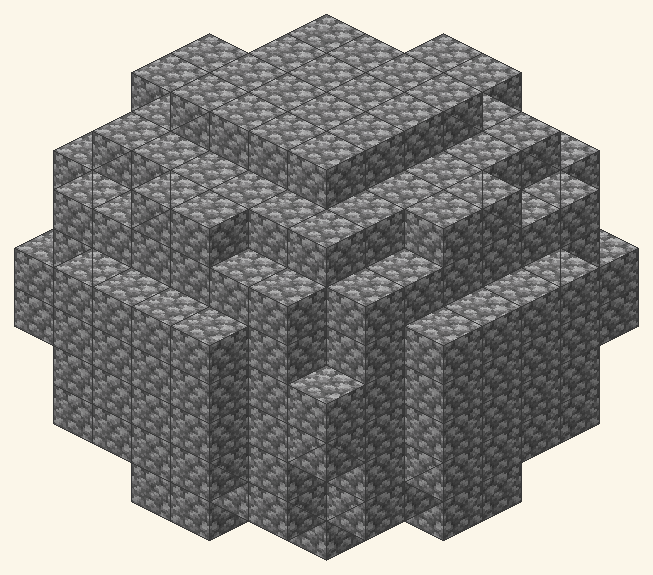
\includegraphics[width=0.55\linewidth]{fig10_3d_sphere_d12.png}\\[0.4em]
    {\sffamily\footnotesize\color{muted}Sphere de diametre~10 voxelisee par Block Round, rendue avec la texture \emph{cobblestone} (pierre rugueuse) de Minecraft.}
  \end{minipage}
  \vspace{0.7cm}\\
  {\color{rule}\rule{0.6\textwidth}{0.6pt}\par}
  \vspace{0.9cm}
  \begin{minipage}{0.82\textwidth}
    \centering\sffamily\small\color{muted}
    \textbf{Domaines articules :} Mathematiques $\cdot$ Arts plastiques et arts numeriques $\cdot$ Numerique et Sciences Informatiques (NSI) $\cdot$ Culture numerique (CRCN/PIX) $\cdot$ Education aux usages ludiques \\[0.4em]
    \textbf{Reperes officiels :} Programme de la specialite Mathematiques (BO du 22~janvier 2019, modifie 2022) $\cdot$ Reforme du lycee 2019 $\cdot$ Baccalaureat general et Grand Oral $\cdot$ \hyperref[sec:olympiades]{Olympiades de Mathematiques} $\cdot$ Minecraft Education
  \end{minipage}
\end{titlepage}

% =============================================================================
\renewcommand{\contentsname}{\color{accent}Sommaire}
\tableofcontents
\thispagestyle{fancy}
\newpage

% =============================================================================
\section{Identification et contextualisation}\label{sec:identificacao}

\begin{center}
\begin{tabular}{@{}p{0.32\textwidth}p{0.62\textwidth}@{}}
\toprule
\textbf{Discipline} & Mathematiques (avec articulation interdisciplinaire forte : Arts plastiques, NSI, Sciences de l'ingenieur, Histoire-Geographie, Sciences economiques et sociales). \\
\addlinespace[2pt]
\textbf{Niveau} & Terminale generale, specialite \emph{Mathematiques} (et, optionnellement, \emph{Mathematiques expertes}). Adaptable en Premiere generale et en Terminale technologique (STI2D, STMG, STL, STD2A). \\
\addlinespace[2pt]
\textbf{Voies couvertes} & Lycee general, lycee technologique (series STI2D, STMG, STL, STD2A), lycee professionnel (Bac~Pro), CFA, lycee agricole, Greta, DAEU et reprise d'etudes pour adultes. \\
\addlinespace[2pt]
\textbf{Volume horaire} & 5~seances de 50~minutes (250~min en classe) + travaux extra-scolaires optionnels. Variante en 2~seances doubles de 100~min decrite en §\ref{sec:adapt}. \\
\addlinespace[2pt]
\textbf{Ressource centrale} & Block Round --- application \emph{web} gratuite, sans inscription, sans serveur, executable hors ligne dans le navigateur (PWA). Conforme au RGPD : ne collecte ni ne transmet aucune donnee personnelle. Fonctionne sur un \emph{smartphone} d'entree de gamme --- ne necessite ni Java, ni installation de Minecraft. \\
\addlinespace[2pt]
\textbf{Blocs du Programme} & Geometrie reperee dans le plan et dans l'espace $\cdot$ Analyse (integration, primitives, volumes) $\cdot$ Algorithmique et programmation (Python). \\
\addlinespace[2pt]
\textbf{Itineraires connexes} & Specialite \emph{Numerique et Sciences Informatiques} (NSI) ; specialite \emph{Sciences de l'ingenieur} (SI) ; \emph{Arts plastiques} et \emph{Arts numeriques} ; option \emph{Mathematiques expertes}. La sequence peut nourrir un projet de \emph{Grand Oral} et une participation aux \hyperref[sec:olympiades]{Olympiades Academiques de Mathematiques}. \\
\addlinespace[2pt]
\textbf{Articulations} & \hyperref[sec:olympiades]{Olympiades Academiques de Mathematiques} $\cdot$ Concours \emph{Castor Informatique} et France-IOI $\cdot$ Concours \emph{Alkindi} $\cdot$ Concours \emph{Kangourou} $\cdot$ Minecraft Education (via Microsoft~365 Education et Reseau Canope). \\
\addlinespace[2pt]
\textbf{Prerequis eleves} & Repere orthonorme du plan ; equation cartesienne du cercle (Premiere) ; aires et volumes des solides usuels (Seconde / Premiere) ; notion de fonction ; proportions et pourcentages ; bases de Python (boucles, conditions, listes). Familiarite avec \emph{Minecraft} : recommandee mais non requise (Block Round s'en passe). \\
\addlinespace[2pt]
\textbf{Preparation de l'enseignant\textperiodcentered e} & 20~minutes d'exploration prealable de Block Round ; lecture de \texttt{docs\_math/Block\_Round\_Math\_fr-FR.pdf} (document technique en francais) ; eventuellement, contact superficiel avec les commandes \cmd{/fill}, \cmd{/clone} et \cmd{//sphere} de Minecraft Java Edition. \\
\bottomrule
\end{tabular}
\end{center}


\begin{note}[Diversite du lycee francais]
Cette sequence a ete concue pour la pluralite des lycees francais : le lycee general en grande metropole (Paris, Lyon, Marseille, Toulouse, Bordeaux) ; le lycee general en chef-lieu de departement ; le lycee technologique en zone industrielle ; le lycee rural des Cevennes, du Cantal, de la Lozere ou de l'Aveyron ; le lycee en Reseau d'Education Prioritaire (REP/REP+) en quartier populaire ; les lycees d'outre-mer (Guyane, Reunion, Polynesie, Nouvelle-Caledonie, Mayotte, Martinique, Guadeloupe) ; les Greta et lycees du soir pour adultes en reprise d'etudes. Chacun de ces contextes appelle des ajustements specifiques, detailles en §\ref{sec:adapt}. Block Round a ete retenu parce qu'il \emph{s'adapte a tous} : il tourne sur \emph{smartphone} d'entree de gamme, se passe d'Internet apres le premier chargement (PWA), ne demande aucune inscription, et ne collecte aucune donnee personnelle --- condition exigee par le RGPD et la loi Informatique et Libertes.
\end{note}

\begin{minecraft}[Pourquoi ancrer la sequence dans Minecraft]
Minecraft est le jeu video le plus vendu de l'histoire (plus de 300~millions d'exemplaires ecoules). En France, c'est une reference culturelle transversale parmi les adolescent\textperiodcentered es, traversant les frontieres sociales que d'autres jeux ne franchissent pas (la version Pocket Edition sur smartphone coute moins de 8~\euro{}, et l'offre \emph{Minecraft Education} est gratuite pour les enseignants verifies via leur adresse academique \texttt{prenom.nom@ac-XXX.fr}). Les etudes de l'ARCEP et du Reseau Canope sur les usages numeriques des adolescents placent regulierement Minecraft parmi les trois jeux les plus cites par les 12--17~ans. \emph{Choisir Minecraft comme point d'ancrage n'est pas une concession a la mode : c'est reconnaitre ou la jeunesse francaise vit deja et fait deja de la geometrie.}
\end{minecraft}

% =============================================================================
\section{Justification pedagogique}\label{sec:justificativa}

Le choix de Block Round comme artefact didactique pour la Terminale specialite Mathematiques repond a une demande \acc{quintuple} de l'enseignement secondaire francais contemporain : integrer mathematiques formelles et culture numerique (CRCN, certification PIX) ; contextualiser le savoir abstrait dans des pratiques \emph{signifiantes} pour l'eleve ; preparer aux epreuves ecrite et orale du Baccalaureat (specialite Mathematiques) et au \emph{Grand Oral}, ou un eleve peut presenter un projet Block Round/Minecraft ; dialoguer avec la reforme du lycee de 2019 (creation des specialites) en articulant Mathematiques et NSI ; et mobiliser l'univers culturel de Minecraft comme passerelle motivationnelle sans perdre en rigueur mathematique.

La \emph{voxel art} occupe une place centrale dans l'imaginaire des adolescent\textperiodcentered es francais\textperiodcentered es. \emph{Minecraft} --- jeu ne en 2009, rachete par Microsoft en 2014 pour 2,5~milliards de dollars, aujourd'hui deploye dans les ecoles via \emph{Minecraft Education} --- est la reference culturelle la plus transversale chez les lyceen\textperiodcentered nes francais\textperiodcentered es. Prendre la construction en voxels comme point de depart transforme une tradition \emph{ludique} familiere en \emph{probleme mathematique authentique} : decrire, sur une grille discrete de blocs $1\times1\times1$, des formes analytiquement definies sur $\mathbb{R}^3$. L'eleve qui construit chaque soir des cubes, des tours, des fermes circulaires et des domes sur le serveur Minecraft de sa classe percoit que ce qu'il fait par intuition porte un nom : \emph{voxelisation}, \emph{rasterisation discrete}, \emph{equation implicite de l'ellipsoide}.

Ce mouvement didactique dialogue avec cinq traditions de la pedagogie francaise et internationale :

\begin{itemize}[leftmargin=1.3em,itemsep=0.2em,topsep=0.3em]
  \item \acc{Celestin Freinet} (1896--1966 ; \emph{L'imprimerie a l'ecole}, 1924 ; \emph{L'education du travail}, 1947). Le point de depart est la culture numerique concrete de l'eleve --- et non l'abstraction de l'equation --- ce qui rapproche la sequence de la pedagogie active freinetienne, du \emph{texte libre} et de la \emph{correspondance scolaire}. Un serveur Minecraft de classe \emph{est} directement freinetien : production cooperative, expression libre, journal de bord, communication entre etablissements. L'eleve qui sait deja construire des spheres dans Minecraft (meme intuitivement) y arrive comme sujet actif, non comme tabula rasa.

  \item \acc{Yves Chevallard} (transposition didactique, 1985 ; theorie anthropologique du didactique --- TAD, Aix-Marseille). Les trois algorithmes de Block Round (Euclidien, Bresenham, Seuil) constituent trois \emph{praxeologies} distinctes pour un meme probleme : trois manieres d'organiser tache, technique, technologie et theorie. Les tutoriels de construction circulaire publies en francais sur YouTube par la communaute Minecraft (Aypierre, Frigiel \& Fluffy, Siphano, Inoxtag) constituent une \emph{quatrieme} praxeologie vernaculaire --- populaire, orale, mediee par le jeu, contemporaine.

  \item \acc{Guy Brousseau} (Theorie des Situations Didactiques --- TSD, Bordeaux). La construction collective du critere de pertinence dans la seance~1 est un exemple paradigmatique de \emph{situation a-didactique} brousseennne : l'eleve se confronte au milieu (la grille discrete) et a ses pairs avant que l'enseignant\textperiodcentered e n'institutionnalise le savoir.

  \item \acc{Philippe Meirieu} (\emph{Apprendre... oui, mais comment ?}, 1987 ; \emph{Faire la classe}, 2004). La defense d'une ecole de la confiance, d'une pedagogie de l'attention et du \emph{learning by doing} structure toutes les activites pratiques. Minecraft pousse a l'extreme le principe deweyen : le joueur teste ses hypotheses constructives en temps reel.

  \item \acc{Ubiratan D'Ambrosio} (Bresil ; \emph{Ethnomathematique}, 1985 sqq. ; ICMI Felix Klein Award, 2005 ; traduit au CNRS). Differentes cultures construisent differents \emph{modes de faire} mathematiques. Cette dimension d'ethnomathematique connecte la sequence aux savoirs vernaculaires francais : architecture en pierre seche des Cevennes et des bories du Vaucluse (voxel manuel par excellence), vitraux gothiques de Notre-Dame de Paris et de Chartres (voxel en verre), tapisserie de Bayeux (rasterisation textile preinformatique du XIe~siecle).
\end{itemize}

La presence du logiciel remplit une fonction epistemique precise : il \emph{ne se substitue pas} a l'algebre, mais \emph{materialise} la difference entre formulations mathematiques concurrentes. Les trois algorithmes correspondent a trois definitions mathematiquement distinctes du meme objet --- le cercle discret --- et produisent des traces visiblement differents, comme l'illustre la Figure~\ref{fig:comp-d10}. L'eleve percoit, par les yeux, que \emph{la definition compte}, et simultanement que le resultat n'est pas abstrait : \emph{il peut construire cela, bloc par bloc, dans Minecraft}.

\begin{figure}[!htbp]
\centering
\begin{subfigure}[t]{0.31\linewidth}\centering
  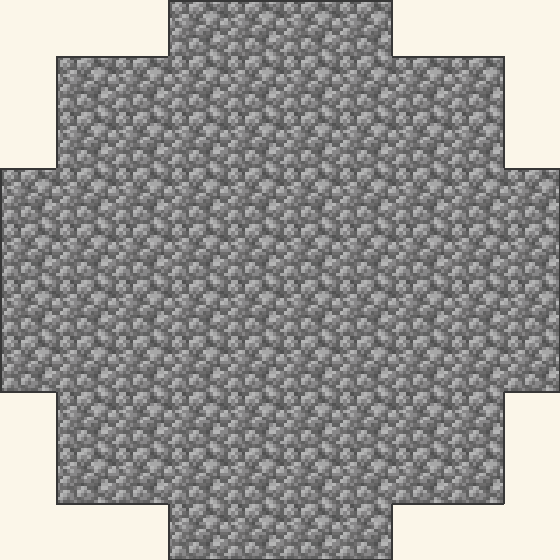
\includegraphics[width=\linewidth]{fig01_2d_d10_euclidean.png}
  \caption{\emph{Euclidien}}
\end{subfigure}\hfill
\begin{subfigure}[t]{0.31\linewidth}\centering
  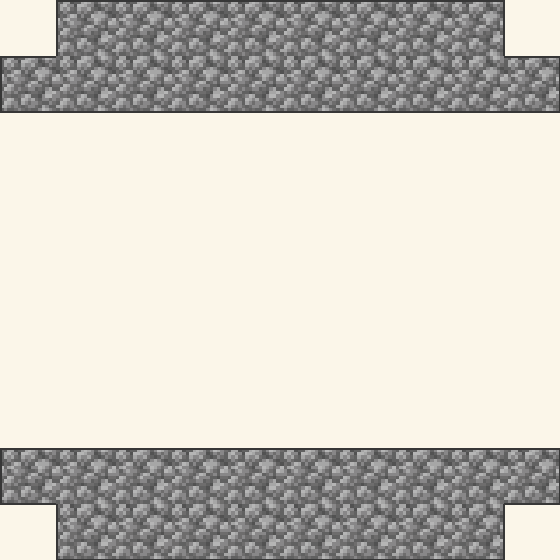
\includegraphics[width=\linewidth]{fig02_2d_d10_bresenham.png}
  \caption{\emph{Bresenham}}
\end{subfigure}\hfill
\begin{subfigure}[t]{0.31\linewidth}\centering
  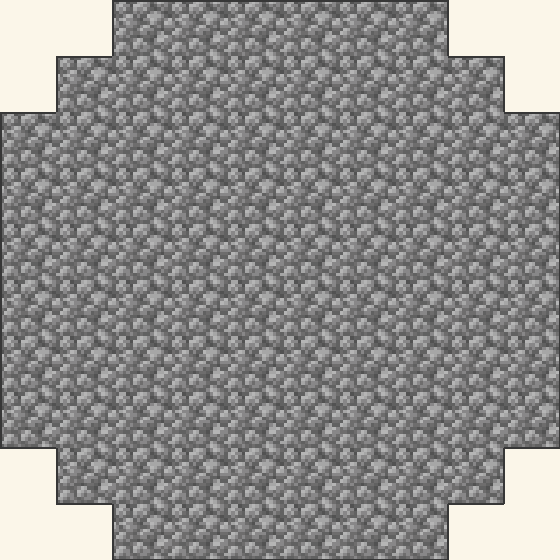
\includegraphics[width=\linewidth]{fig03_2d_d10_threshold.png}
  \caption{\emph{Seuil}}
\end{subfigure}
\caption{Un meme cercle de diametre~10 sous trois criteres de pertinence, rendu avec la texture \emph{cobblestone} (pierre rugueuse) de Minecraft. Observez comme les cellules de coin, la transition entre rangees et les points cardinaux varient d'une version a l'autre --- ce sont trois reponses \emph{mathematiquement correctes} sous des criteres distincts, et trois plans de construction differents dans \emph{Minecraft}.}
\label{fig:comp-d10}
\end{figure}

\begin{note}[Equite et realite materielle du lycee francais]
Le choix de Block Round repond, en partie, a un probleme materiel concret : les inegalites d'acces aux ressources numeriques entre lycees. La Direction du Numerique pour l'Education (DNE) et les rapports de l'ARCEP indiquent que la dotation en salles informatiques varie sensiblement selon les academies (urbain dense, peripheries, ruralite). En revanche, le taux d'equipement personnel en \emph{smartphone} chez les 15--18~ans depasse 95~\% sur tout le territoire (INSEE, Reseau Canope). Block Round a ete concu exactement pour ce scenario : \emph{smartphone} d'entree de gamme, sans connexion permanente, sans compte --- et, si besoin, l'Annexe~\ref{ap:adapt-analog} propose un itineraire \emph{entierement analogique} sur papier quadrille. \emph{Minecraft Pocket Edition tourne sur des smartphones de trois ans d'age} : l'eleve peut commencer en classe sur Block Round et continuer chez lui sur Minecraft.
\end{note}

\begin{minecraft}[Recherche : Minecraft a l'ecole francaise]
Plusieurs experimentations recentes documentent l'usage pedagogique de Minecraft en France : le \emph{Reseau Canope} mene des formations Minecraft Education et publie des scenarios sur \url{https://www.reseau-canope.fr/} ; l'INRIA (programmes \emph{Pixees}, \emph{1, 2, 3, Codez} de la Fondation La main a la pate) integre Minecraft dans ses ressources d'enseignement de l'informatique ; plusieurs academies (Paris, Lyon, Versailles, Aix-Marseille) ont signe des accords-cadres avec Microsoft Education pour deployer Minecraft Education dans leurs lycees pilotes. Cette sequence complete cette tradition : elle utilise Block Round comme \emph{passerelle} vers Minecraft, en dispensant de l'installation du jeu au moment du cours.
\end{minecraft}

% =============================================================================
\section{Objectifs}\label{sec:objetivos}

\subsection{Objectif general}

Conduire les eleves a \acc{comprendre, comparer, utiliser et traduire-en-construction} les definitions formelles du cercle, de l'ellipse et de l'ellipsoide comme criteres d'inclusion de cellules sur une grille discrete de voxels textures, en mobilisant l'equation implicite de ces figures pour expliquer, prevoir, modifier et \emph{construire dans Minecraft} des productions visuelles auctoriales, en dialogue avec le patrimoine architectural francais (gothique, classique, modernite) et avec la tradition mathematique nationale. La conscience de cette pluralite de reponses valides s'inscrit dans une culture mathematique francaise qui a vu, en 2022, \hyperref[sec:olympiades]{Hugo Duminil-Copin} recevoir a 36~ans la Medaille Fields, et qui voit les communautes francaises de \emph{Minecraft} construire chaque jour des cites entieres en articulant geometrie spatiale, sans necessairement la nommer.

\subsection{Objectifs specifiques}

\textbf{Cognitifs (conceptuels) :}
\begin{itemize}[leftmargin=1.3em,itemsep=0.2em,topsep=0.3em]
  \item identifier l'equation implicite $\left(\dfrac{x}{r_x}\right)^{\!2} + \left(\dfrac{y}{r_y}\right)^{\!2} = 1$ comme cas general contenant le cercle $x^2 + y^2 = r^2$ ;
  \item reconnaitre que trois criteres distincts de pertinence (distance au centre, point milieu de Bresenham, couverture de coin) produisent trois ensembles differents de cellules --- comme deja vu sur la Figure~\ref{fig:comp-d10} ;
  \item comprendre la transition de l'equation 2D a l'equation 3D de l'ellipsoide et la mettre en relation avec le calcul du volume $V = \tfrac{4}{3}\pi r_x r_y r_z$ (sujet recurrent dans le bloc \emph{Analyse} du programme de specialite et dans l'epreuve ecrite du Baccalaureat) ;
  \item interpreter la coupe d'un solide par un plan comme une \emph{inegalite lineaire} appliquee aux coordonnees des voxels ;
  \item comprendre l'\emph{arithmetique de l'inventaire Minecraft} (piles de~64, coffres simples de 27~emplacements, coffres doubles de 54~emplacements) comme application concrete de la \emph{division entiere avec quotient et reste} et du \emph{plafond} ($\lceil \cdot \rceil$) ;
  \item identifier les \emph{symetries} (reflexion, rotation) qui permettent de construire une sphere complete a partir d'un octant par la commande \cmd{/clone}.
\end{itemize}

\textbf{Procedural :}
\begin{itemize}[leftmargin=1.3em,itemsep=0.2em,topsep=0.3em]
  \item manipuler l'interface de Block Round dans ses deux modes (2D et 3D) et exporter images en PNG et schematics au format \texttt{.schem} ;
  \item tracer manuellement, sur papier quadrille, l'approximation discrete d'un cercle en appliquant le critere euclidien, puis la verifier dans le logiciel ;
  \item calculer l'aire / le volume discret d'une figure voxelisee en comptant les cellules et comparer avec l'aire / le volume continu, en exprimant le resultat sous forme d'erreur relative ;
  \item composer une figure auctoriale combinant cercles, ellipses et ellipsoides avec justification mathematique des choix, en prevoyant le nombre de blocs par type et la quantite de coffres doubles necessaires ;
  \item importer un schematic exporte par Block Round dans Litematica ou Schematica (mods Minecraft) et executer la construction dans le jeu ;
  \item ecrire une sequence de commandes \cmd{/clone} reflectant un octant en une sphere complete.
\end{itemize}

\textbf{Attitudinaux :}
\begin{itemize}[leftmargin=1.3em,itemsep=0.2em,topsep=0.3em]
  \item cooperer en binomes ou trinomes dans la production des activites pratiques, simulant des equipes de \emph{builders} de serveur Minecraft ;
  \item argumenter mathematiquement en faveur d'un choix esthetique --- competence directement evaluee lors du \emph{Grand Oral} du Baccalaureat ;
  \item reconnaitre que les problemes reels (y compris celui de \enquote{construire une coupole de Quartz sur le serveur de la classe}) admettent plus d'une reponse techniquement correcte ;
  \item identifier des references mathematiques dans le patrimoine culturel francais, dans les savoirs vernaculaires (architecture en pierre seche, gothique, modernite) et dans la production numerique contemporaine ;
  \item developper une \emph{ethique numerique} : respecter le travail des camarades, citer la source des \emph{builds} reutilisees, comprendre la notion de licence libre.
\end{itemize}


% =============================================================================
\section{Programme de la specialite Mathematiques et competences mobilisees}\label{sec:bncc}

La sequence mobilise directement \acc{quatre blocs} du programme de la specialite Mathematiques en classe terminale (BO du 22~janvier 2019, modifie 2022), ainsi que les six \emph{competences mathematiques} (chercher, modeliser, representer, raisonner, calculer, communiquer).

\begin{competence}[Geometrie reperee dans l'espace]
Reperer un point de l'espace par ses coordonnees dans un \acc{repere orthonorme} ; calculer la \acc{distance entre deux points} ; etablir et utiliser l'\emph{equation cartesienne} d'une sphere et l'\emph{equation parametrique} d'une droite ou d'un plan. Resolution de problemes faisant intervenir \emph{des configurations dans l'espace}.
\end{competence}

\begin{competence}[Equations cartesiennes du plan et du cercle (rappel Premiere)]
Equation cartesienne d'un cercle de centre $\Omega(a, b)$ et de rayon $r$ : $(x - a)^2 + (y - b)^2 = r^2$. \acc{Equation reduite} de l'ellipse $\dfrac{x^2}{a^2} + \dfrac{y^2}{b^2} = 1$, traitee comme transformation lineaire du cercle unite.
\end{competence}

\begin{competence}[Analyse --- Integration et volumes]
Notion de \acc{primitive} ; \emph{integrale} d'une fonction continue et positive ; \acc{volume} d'un solide de revolution ; volume de la sphere $V = \tfrac{4}{3}\pi r^3$ et de l'ellipsoide $V = \tfrac{4}{3}\pi r_x r_y r_z$ ; \emph{approximation numerique} par discretisation.
\end{competence}

\begin{competence}[Algorithmique et programmation (Python)]
Conception et \acc{implementation d'algorithmes} elementaires en Python : boucles \texttt{for}, instructions conditionnelles, listes et tableaux \emph{NumPy}. Lecture critique d'un code : comprendre, executer mentalement, modifier. Implementation des trois algorithmes Euclidien, Bresenham et Seuil.
\end{competence}

\medskip
Sont egalement mobilisees les \emph{six competences mathematiques} :

\begin{itemize}[leftmargin=1.3em,itemsep=0.15em,topsep=0.3em]
  \item \acc{Chercher} --- engager une demarche d'exploration sur la grille discrete ;
  \item \acc{Modeliser} --- traduire un objet ludique (le bloc Minecraft) en objet mathematique (le voxel) ;
  \item \acc{Representer} --- passer d'un registre a l'autre (algebrique, geometrique, computationnel, voxel) ;
  \item \acc{Raisonner} --- justifier la correction d'un algorithme et la borne de l'erreur relative ;
  \item \acc{Calculer} --- evaluer volumes continus et discrets, faire l'arithmetique des piles ;
  \item \acc{Communiquer} --- argumenter ses choix, en particulier lors du Grand Oral.
\end{itemize}

\subsection{Articulation avec le Baccalaureat (specialite Mathematiques)}\label{sec:bac}

Les competences mobilisees plus haut se retrouvent dans plusieurs descripteurs des sujets recurrents au Baccalaureat de la specialite Mathematiques :

\begin{itemize}[leftmargin=1.3em,itemsep=0.15em,topsep=0.3em]
  \item \emph{Geometrie reperee} : equations de droites, plans, spheres dans l'espace ; produits scalaires ; orthogonalite. Sujets recurrents en juin et septembre.
  \item \emph{Analyse} : primitives, integrales, volumes de solides de revolution. Tres frequent.
  \item \emph{Algorithmique et programmation Python} : un exercice systematique du sujet ecrit demande lire/completer/executer un code Python.
  \item \emph{Grand Oral} : un\textperiodcentered e eleve peut presenter, en specialite Mathematiques, le projet \emph{Block Round + Minecraft} comme son sujet, articulant l'algorithme de Bresenham, le volume de l'ellipsoide et l'application en construction reelle.
\end{itemize}

Les modalites officielles du Baccalaureat 2025 sont consultables sur \url{https://eduscol.education.fr/}.

\subsection{Culture numerique --- CRCN et certification PIX}

Le \emph{Cadre de Reference des Competences Numeriques} (CRCN) structure quatre des cinq domaines des competences PIX traverses par la sequence : \emph{informations et donnees}, \emph{communication et collaboration}, \emph{creation de contenus}, \emph{environnement numerique}. La sequence permet aux eleves d'atteindre les niveaux PIX requis pour la certification en fin de Terminale (niveau~5 a 6 selon les domaines). Sont discutees les questions d'\emph{ethique numerique} (licences libres versus logiciels proprietaires ; Microsoft autorise l'usage educatif gratuit de Minecraft via Education Edition), de \emph{protection des donnees personnelles} (\href{https://www.cnil.fr/fr/reglement-europeen-protection-donnees}{RGPD, Reglement UE 2016/679} et Loi Informatique et Libertes modifiee en 2018, sous controle de la CNIL --- Block Round ne stocke rien), de \emph{production autoriale} (droits sur les creations des eleves en Seance~\ref{aula5}) et de \emph{citoyennete numerique} (comportement responsable sur serveurs Minecraft, prevention du \emph{griefing} et du cyberharcelement).

% =============================================================================
\section{Contenus}\label{sec:conteudos}

\subsection{Notionnels}
\begin{itemize}[leftmargin=1.3em,itemsep=0.15em,topsep=0.3em]
  \item Repere orthonorme et systeme de coordonnees dans $\mathbb{R}^2$ et $\mathbb{R}^3$ ; centre de cellule \emph{vs.} coin.
  \item Equation cartesienne du cercle : $x^2 + y^2 = r^2$ ; equation reduite generale du cercle de centre $\Omega(a, b)$.
  \item Equation implicite generale de l'ellipse : $\left(\dfrac{x}{r_x}\right)^{\!2} + \left(\dfrac{y}{r_y}\right)^{\!2} = 1$.
  \item Inegalite de pertinence : \emph{interieur, exterieur} et \emph{frontiere}.
  \item Equation de l'ellipsoide et de la sphere dans $\mathbb{R}^3$.
  \item Volume continu de l'ellipsoide : $V = \tfrac{4}{3}\pi r_x r_y r_z$, etabli via une integrale double / triple en \emph{Mathematiques expertes}.
  \item Plans de l'espace comme \emph{inegalites lineaires} (operation de coupe).
  \item Voisinage d'une cellule (4-connecte en 2D, 6-connecte en 3D).
  \item \acc{Arithmetique de l'inventaire Minecraft} : piles de~64 ; coffres simples (27~emplacements) et coffres doubles (54~emplacements) ; division avec plafond $N_{\mathrm{piles}} = \lceil N/64 \rceil$.
  \item \acc{Symetrie octaedrique} et groupe $\mathbb{Z}_2^3$ des reflexions de coordonnees (sous-groupe d'ordre~8 de $O_h$) : application en construction optimisee via \cmd{/clone}.
\end{itemize}

\subsection{Procedural}
\begin{itemize}[leftmargin=1.3em,itemsep=0.15em,topsep=0.3em]
  \item Trace manuel sur papier quadrille selon un critere explicite.
  \item Manipulation de Block Round (changement de mode, ajustement des \emph{sliders}, choix d'algorithme, exportation en PNG et \texttt{.schem}).
  \item Comparaison d'aires / volumes discrets et continus par comptage.
  \item Composition de figures combinees (\emph{voxel art} auctoriale avec justification geometrique).
  \item Importation de \texttt{.schem} dans Litematica / Schematica.
  \item Execution de commandes vanilla \cmd{/fill}, \cmd{/clone}, \cmd{/setblock} et WorldEdit \cmd{//sphere}, \cmd{//hsphere}, \cmd{//ellipsoid}.
  \item Implementation Python des trois algorithmes (rapprochement direct avec la specialite NSI).
  \item Planification de la collecte de ressources en mode \emph{survie}.
\end{itemize}

\subsection{Attitudinaux}
\begin{itemize}[leftmargin=1.3em,itemsep=0.15em,topsep=0.3em]
  \item Travail cooperatif en binomes ou trinomes.
  \item Argumentation fondee (justifier les choix avec des mathematiques).
  \item Ethique numerique : respect de la licence du logiciel, des productions des camarades et des regles du serveur Minecraft partage.
  \item Valorisation des references mathematiques presentes dans le patrimoine francais et dans la culture \emph{gamer} contemporaine.
\end{itemize}

\subsection{Modes de rendu et variete d'algorithmes}

Outre le changement d'algorithme, Block Round offre trois \emph{modes de rendu} (Plein, Mince, Epais) qui produisent des resultats visuels distincts pour la meme figure geometrique, comme l'illustre la Figure~\ref{fig:render-modes}. Dans Minecraft, ces modes correspondent a trois types de construction distincts : une sphere \emph{Pleine} utilise tous les blocs de l'interieur (une coupole opaque en \emph{Stone}) ; \emph{Mince} ne montre que la coque (une coupole \emph{creuse}, vide a l'interieur pour une salle ou un musee) ; \emph{Epaisse} ferme les fentes diagonales que le mode Mince laisse (\emph{essentielle} pour les coupoles en \emph{Verre} ou en \emph{Glace} sous-marines qui doivent etre etanches).

\begin{figure}[!htbp]
\centering
\begin{subfigure}[t]{0.31\linewidth}\centering
  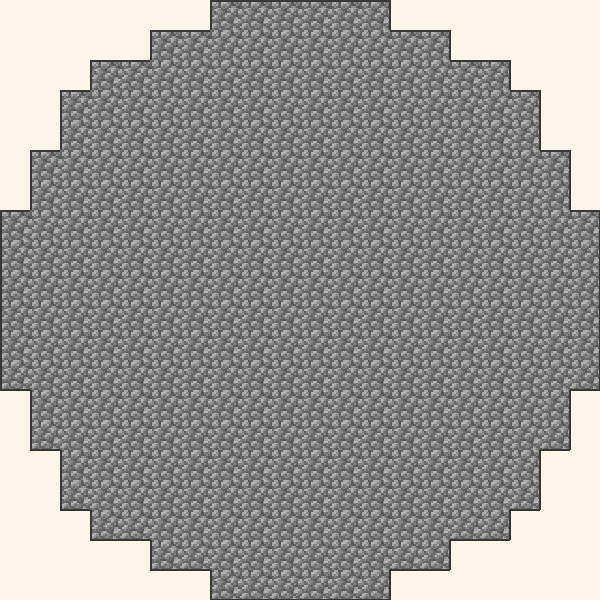
\includegraphics[width=\linewidth]{fig04_2d_d20_euclidean.png}
  \caption{\emph{Plein}}
\end{subfigure}\hfill
\begin{subfigure}[t]{0.31\linewidth}\centering
  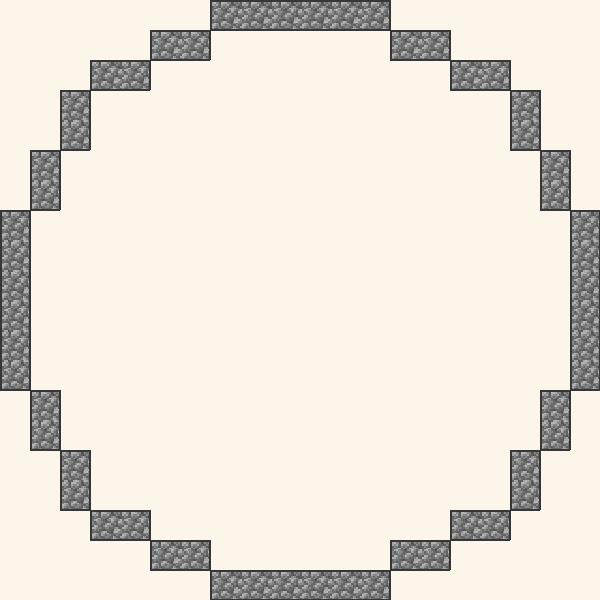
\includegraphics[width=\linewidth]{fig08_2d_d20_thin.png}
  \caption{\emph{Mince} (contour de 1~bloc)}
\end{subfigure}\hfill
\begin{subfigure}[t]{0.31\linewidth}\centering
  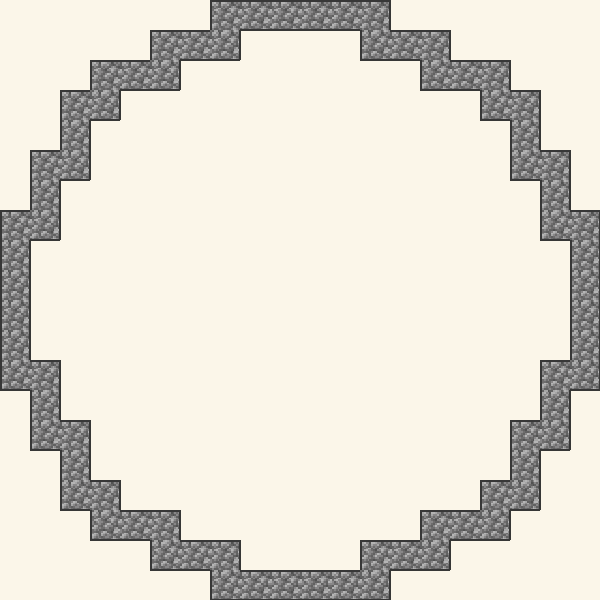
\includegraphics[width=\linewidth]{fig09_2d_d20_thick.png}
  \caption{\emph{Epais} (contour avec ponts diagonaux)}
\end{subfigure}
\caption{Les trois modes de rendu pour le meme cercle euclidien de diametre~20. Le mode \emph{Mince} correspond au bord discret topologique ; le mode \emph{Epais} ajoute des blocs sur les diagonales pour eviter les trous a $45^\circ$ --- exactement le probleme qui apparait sur une coupole en Verre sous-marine de Minecraft, ou une fente diagonale laisse passer l'eau.}
\label{fig:render-modes}
\end{figure}

\subsection{Textures de bloc : le marqueur Block Round}

Bien que la mathematique de \emph{quels voxels poser} soit independante de la texture, Block Round rend chaque voxel avec sa texture canonique a six faces de Minecraft. La meme sphere de diametre~10 change completement de caractere visuel selon le bloc choisi (Figure~\ref{fig:textures}), \emph{sans aucun changement dans l'algorithme} sous-jacent. C'est le point pedagogique central : la \emph{forme} est issue des mathematiques, l'\emph{apparence} est une decision esthetique a posteriori.

\begin{figure}[!htbp]
\centering
\begin{subfigure}[t]{0.31\linewidth}\centering
  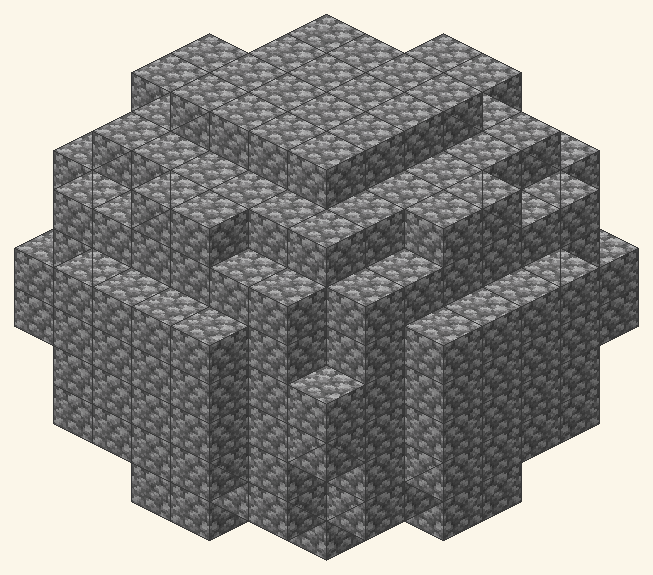
\includegraphics[width=\linewidth]{fig15_3d_sphere_cobblestone.png}
  \caption{\emph{Cobblestone}}
\end{subfigure}\hfill
\begin{subfigure}[t]{0.31\linewidth}\centering
  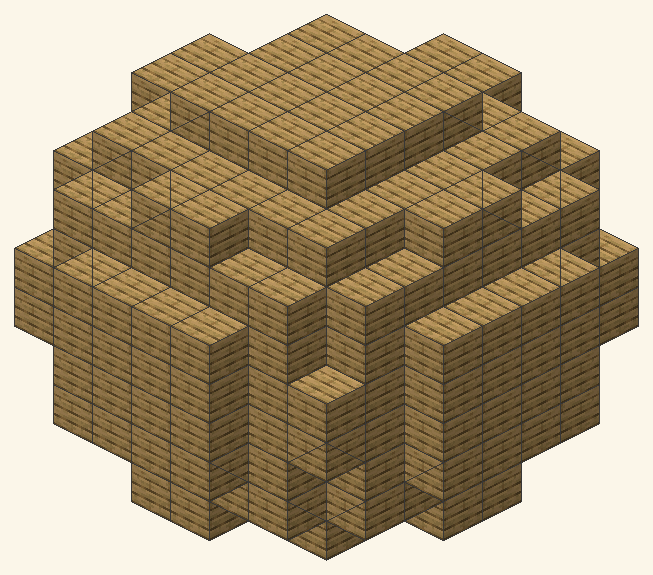
\includegraphics[width=\linewidth]{fig17_3d_sphere_oak.png}
  \caption{\emph{Oak Planks}}
\end{subfigure}\hfill
\begin{subfigure}[t]{0.31\linewidth}\centering
  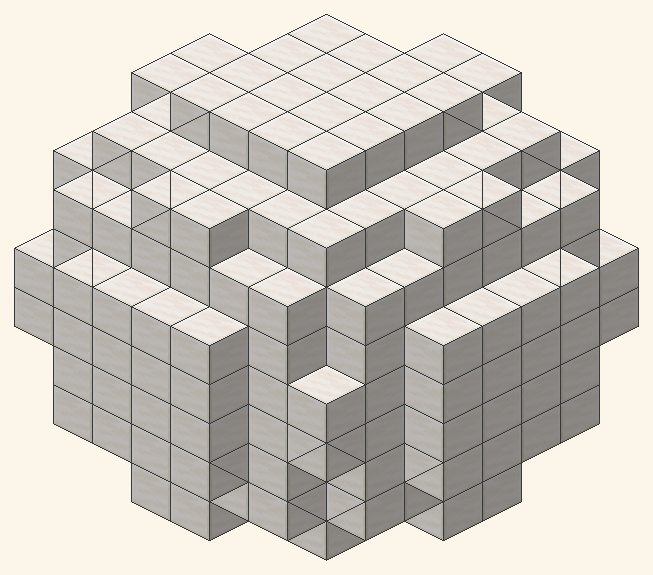
\includegraphics[width=\linewidth]{fig19_3d_sphere_quartz.png}
  \caption{\emph{Quartz Block}}
\end{subfigure}
\caption{Trois textures Minecraft appliquees a la \emph{meme} sphere de diametre~10. La silhouette voxelisee est identique dans les trois versions --- la mathematique n'a pas change. Ce qui change, c'est le caractere visuel : \emph{Cobblestone} suggere une muraille medievale, \emph{Oak Planks} suggere l'interieur d'une cabane ou d'un navire, \emph{Quartz Block} suggere un temple moderne.}
\label{fig:textures}
\end{figure}

% =============================================================================
\section{Prerequis}\label{sec:prerrequisitos}

La sequence presuppose des connaissances anterieures sur :

\begin{itemize}[leftmargin=1.3em,itemsep=0.15em,topsep=0.3em]
  \item Repere orthonorme : reperage de points $(x, y)$ et $(x, y, z)$.
  \item Equation reduite du cercle (programme de Premiere generale, specialite Mathematiques).
  \item Aires des polygones et du disque ; volumes du cube, du pave droit, du prisme et du cylindre (programme de Seconde et Premiere).
  \item Notion de fonction : domaine, image, courbe representative.
  \item Notions de proportion et de pourcentage.
  \item Division euclidienne avec quotient et reste (programme de college).
  \item Bases de Python : variables, boucle \texttt{for}, instruction conditionnelle, listes, tableaux \emph{NumPy} (programme de specialite Mathematiques et NSI).
\end{itemize}

\emph{Prerequis optionnel (non requis, mais utile) :} familiarite avec Minecraft. Cette sequence a ete deliberement concue pour que meme un\textperiodcentered e eleve qui n'a \emph{jamais} joue a Minecraft (situation rare mais possible, notamment en lycee rural a faible connectivite) puisse suivre pleinement --- toute l'operation se passe sur Block Round, qui est \emph{auto-contenu} dans le navigateur.

Si la classe presente des lacunes sur certains des points obligatoires ci-dessus --- realite frequente post-pandemie, qu'attestent les evaluations nationales de la DEPP parues entre 2021 et 2024 et publiees sur \href{https://www.education.gouv.fr/}{eduscol.education.gouv.fr} --- la \emph{Seance~1} prevoit un moment de \emph{diagnostic} (10~min) decrit en §\ref{aula1}.

% =============================================================================
\section{Ressources et materiels}\label{sec:recursos}

\subsection{Ressources numeriques}
\begin{itemize}[leftmargin=1.3em,itemsep=0.15em,topsep=0.3em]
  \item Block Round (une instance par eleve \emph{ou} par binome) ;
  \item Videoprojecteur, TV avec entree HDMI ou tableau numerique interactif (TBI / VPI) ;
  \item Acces a une \emph{salle informatique} \emph{ou} utilisation des \emph{smartphones} personnels (BYOD --- \emph{Bring Your Own Device}) \emph{ou} \emph{tablettes} pretees par la region (Hauts-de-France, Ile-de-France, Auvergne-Rhone-Alpes mettent regulierement des tablettes a disposition des lyceens) ;
  \item (Optionnel, Seance~\ref{aula5}) acces a Minecraft Java Edition ou Minecraft Education avec les mods \emph{Litematica} ou \emph{Schematica} installes ; alternativement, usage vanilla avec \cmd{/fill} et \cmd{/clone}.
\end{itemize}

\subsection{Ressources analogiques}
\begin{itemize}[leftmargin=1.3em,itemsep=0.15em,topsep=0.3em]
  \item Papier quadrille (1~cm), 2~feuilles par eleve ;
  \item Crayon a papier, gomme, regle de 30~cm ;
  \item Crayons de couleur ou feutres (de preference vert-herbe \texttt{\#5B8E3F} et marron-terre \texttt{\#825432}, palette Block Round) ;
  \item Feuille d'exercices (Annexe~\ref{ap:exerc}) ;
  \item Tableau blanc ou tableau noir.
\end{itemize}

\subsection{Manuel scolaire et programme officiel}\label{sec:pnld}

Block Round complete --- ne remplace pas --- le manuel de specialite Mathematiques adopte par le lycee. Les principales collections francaises couvrent les contenus mobilises :

\begin{itemize}[leftmargin=1.3em,itemsep=0.1em,topsep=0.2em,nosep]
  \item \emph{Mathematiques Terminale specialite}, collection \emph{Indice} (Bordas) ;
  \item \emph{Mathematiques Terminale specialite}, collection \emph{Barbazo} (Hachette Education) ;
  \item \emph{Mathematiques Terminale specialite}, collection \emph{Declic} (Hachette) ;
  \item \emph{Mathematiques Terminale specialite}, collection \emph{Maths Repere} (Hachette) ;
  \item \emph{Mathematiques Terminale specialite}, collection \emph{Transmath} (Nathan).
\end{itemize}

Les chapitres consacres a l'\emph{equation du cercle}, aux \emph{coniques}, a la \emph{geometrie spatiale} (volumes) et au bloc \emph{Algorithmique et programmation} dialoguent directement avec la sequence. En particulier, les problemes de \emph{pavage}, \emph{couverture} et \emph{denombrement sur des grilles} (frequents dans les manuels) sont quasiment identiques au probleme central de Block Round, seulement avec une terminologie differente.

\subsection{Acces a Block Round}

Par ordre de preference :

\begin{enumerate}[leftmargin=1.5em,itemsep=0.15em,topsep=0.3em]
  \item \textbf{Heberge par l'enseignant\textperiodcentered e} sur \emph{GitHub Pages} ou sur le portail de l'etablissement (URL distribuee via QR Code projete au tableau). Version publique : \url{https://vinisouza128.github.io/block-round/}.
  \item \textbf{Copie locale} des fichiers du projet dans un dossier de la salle informatique, executee via \emph{file://}.
  \item \textbf{Hors ligne sur \emph{smartphone}} via PWA : il suffit d'ouvrir une fois avec Internet pour que le navigateur installe l'application.
\end{enumerate}


% =============================================================================
\section{Adaptations a la pluralite du lycee francais}\label{sec:adapt}

Le lycee francais est pluriel --- entre les grandes metropoles, les chefs-lieux de departement, les zones rurales, les REP+, les outre-mers et les Greta pour adultes, les conditions materielles, sociales et culturelles varient considerablement. Cette sequence a ete concue pour s'adapter a cette pluralite, avec des variantes specifiques pour chaque contexte.

\subsection{Lycee general en grande metropole}
Scenario typique des academies de Paris, Lyon, Marseille, Toulouse, Bordeaux et Lille. Dispose en general d'une salle informatique fonctionnelle, d'un tableau numerique interactif et d'une connexion Wi-Fi correcte. Plusieurs etablissements ont des licences \emph{Microsoft~365 Education} qui incluent \emph{Minecraft Education} --- la Seance~\ref{aula5} peut alors etre realisee integralement dans cette version. \emph{Configuration la plus simple pour mettre en oeuvre la sequence integralement en salle.}

\subsection{Lycee general en ville moyenne / chef-lieu}
Realite de la grande majorite des etablissements en France metropolitaine (chefs-lieux de departement comme Chartres, Bourges, Limoges, Albi, Mende, Tulle, Le Puy-en-Velay, Carcassonne). La salle informatique peut etre partiellement fonctionnelle. On recommande le \emph{BYOD} avec smartphones personnels, organises en binomes (un telephone par binome). Block Round tourne sans probleme sur Android a partir de 2018. Si Minecraft n'est pas disponible, la Seance~\ref{aula5} peut se concentrer sur des commandes hypothetiques (papier + description de l'effet) sans perdre le contenu conceptuel. C'est la configuration \acc{la plus courante} en France.

\subsection{Lycee technologique (STI2D, STMG, STL, STD2A) --- itineraire STEAM}
Series technologiques : Sciences et Technologies de l'Industrie et du Developpement Durable (STI2D), Sciences et Technologies du Management et de la Gestion (STMG), Sciences et Technologies de Laboratoire (STL), Sciences et Technologies du Design et des Arts Appliques (STD2A). Bien equipees techniquement. La sequence s'integre naturellement aux enseignements technologiques : \emph{Innovation Technologique} et \emph{Ingenierie et Developpement Durable} (STI2D), \emph{Sciences Physiques et Chimiques en Laboratoire} (STL), \emph{Design et Metiers d'Art} (STD2A). On recommande d'approfondir la Seance~\ref{aula2} (algorithme de Bresenham) avec une implementation Python en salle, et la Seance~\ref{aula5} avec l'installation d'un veritable serveur Minecraft Java pour la construction collaborative. Cas particulier : la serie \emph{STD2A} se prete admirablement a un projet \emph{Design Voxel}, articulant Block Round avec les enseignements de \emph{Design et Arts Appliques}.

\subsection{Lycee rural / territoires ruraux peu denses}
Cas des lycees agricoles (depend du Ministere de l'Agriculture, MAA) et des lycees generaux dans les departements faiblement urbanises (Cantal, Lozere, Creuse, Aveyron, Ariege, Hautes-Alpes, Lot, Indre). Connectivite parfois plus faible ; equipement informatique inegal mais avec une \emph{forte culture pratique} des eleves (constructions agricoles, charpente, hangars, silos). On recommande la variante analogique (Annexe~\ref{ap:adapt-analog}) et un unique appareil de l'enseignant\textperiodcentered e pour demonstration. La Seance~\ref{aula3} peut tirer parti des connaissances des eleves sur les constructions agricoles circulaires (silos, abreuvoirs, ronds de longe) pour articuler geometrie vecue et geometrie symbolique. Articulation possible avec les Maisons Familiales Rurales (MFR) et les CFA agricoles.

\subsection{Lycee en REP/REP+ ou Cite Educative (quartier populaire)}
\href{https://www.education.gouv.fr/}{Reseau d'Education Prioritaire} : etablissements implantes dans des quartiers populaires avec moyens humains et financiers renforces. Programme \emph{Cite Educative} (depuis 2019) pour les territoires les plus fragiles. La sequence se prete particulierement bien a un \emph{projet collectif} de fin de Terminale, mobilisant le serveur Minecraft de la classe comme \enquote{atelier numerique} valorise dans le cadre du Pass Culture (15--18~ans), du Pass Sport et de la \emph{Bourse au merite}. Les associations d'education populaire (Reseau Canope, AFEV, Frateli/Article~1) sont des partenaires naturels pour des projets extra-scolaires en aval de la sequence.

\subsection{Lycees d'outre-mer (DROM-COM)}
Cas des academies de la Guyane, de la Martinique, de la Guadeloupe, de la Reunion, de Mayotte ; des vice-rectorats de la Polynesie francaise et de la Nouvelle-Caledonie ; et de Saint-Pierre-et-Miquelon. La \href{https://www.education.gouv.fr/}{circulaire sur l'enseignement des langues regionales} et l'autochtonite en outre-mer ouvre un champ d'enrichissement culturel considerable : en Guyane, dialogue avec les architectures vernaculaires des communautes amerindiennes Wayanas et Wayampi et avec les cases creoles ; en Polynesie, articulation avec les \emph{fare} (cases traditionnelles, toits coniques en niau ou pandanus --- voxelisation tropicale par excellence) ; en Nouvelle-Caledonie, dialogue avec les \emph{cases kanak} (geometrie en cone tronque, charpente en bambou). Pour Mayotte et la Reunion, valoriser les techniques de construction creoles et mahoraises. \emph{Le professeur\textperiodcentered e d'Histoire-Geographie et le\textperiodcentered la professeur\textperiodcentered e de Langues Vivantes Regionales sont des partenaires precieux dans ces academies.}

\subsection{Adultes en reprise d'etudes (Greta, DAEU, AFPA)}
\emph{Groupements d'Etablissements} (Greta), \emph{Diplome d'Acces aux Etudes Universitaires} (DAEU --- equivalent du Baccalaureat pour adultes), \emph{Agence Formation Professionnelle Adultes} (AFPA), \emph{Lycees du soir} (cours du soir municipaux). Public typiquement adulte revenant a l'ecole. Block Round fonctionne bien parce que l'interface est conviviale et que le theme (Minecraft, jeux video) est aussi familier a cette tranche d'age (de nombreux trentenaires et quadragenaires francais ont grandi avec Minecraft a partir de 2011 ; d'autres l'ont decouvert grace a leurs enfants). On suggere de reduire le temps de chaque activite de 20~\% (en raison des horaires plus courts du soir) et de privilegier les discussions orales plutot que la production ecrite longue. La Seance~\ref{aula5} peut etre rendue \emph{optionnelle} pour les adultes, en se concentrant sur les Seances~1--4.

\subsection{Variante en 2 seances doubles (100~min chacune)}
Pour les lycees qui pratiquent les \emph{modules doubles} (frequents en STI2D, STL et dans les classes a projet pluridisciplinaire) : Seances~1+2 dans un module, 3+4 dans l'autre, Seance~5 seule (ou en module simple de 50~min, ou en module double si l'on a le temps pour la construction reelle). Total : 3~modules de 100~min + 1~module de 50~min, ou 2~modules de 100~min + 1~module double (200~min) pour la partie pratique finale dans Minecraft.

\subsection{Variante hybride / distance}
La nature \emph{web} de Block Round le rend trivialement compatible avec un cours a distance (\emph{Mon Bureau Numerique} des academies, \emph{Pronote}, \emph{ENT régional}, \emph{Microsoft Teams Education}, \emph{Zoom}). L'enseignant\textperiodcentered e partage son ecran ; les eleves suivent sur leur propre machine. Les activites en papier quadrille peuvent etre photographiees et envoyees comme devoir asynchrone via l'ENT ou la plateforme Canope. La Seance~\ref{aula5} peut etre realisee sur un serveur Minecraft partage --- \emph{Realms} ou serveur propre --- la classe se retrouvant dans le monde virtuel pour construire collaborativement.

\subsection{Tableau de croisement avec les academies}

Chaque academie decline le programme national avec ses propres priorites et ses propres ressources pedagogiques. Les principales academies :

\begin{center}
\small
\begin{tabularx}{\textwidth}{@{}p{0.20\textwidth}p{0.24\textwidth}X@{}}
\toprule
\textbf{Academie} & \textbf{Specificite locale} & \textbf{Application de la sequence} \\
\midrule
Paris & Reseau \emph{Maisons Numeriques}, partenariats Microsoft Education et Canope. & Sequence integrale en salle informatique ; Seance~\ref{aula5} en Minecraft Education. \\
\addlinespace[3pt]
Lyon & Accord-cadre Microsoft Education ; reseau \emph{Pixees} de l'INRIA actif. & Articulation NSI + Maths ; projet pour le Grand Oral. \\
\addlinespace[3pt]
Aix-Marseille & IREM tres actif (Aix, Marseille) ; CIRM de Luminy. & Ressource pour formation continue PNF (Plan National de Formation). \\
\addlinespace[3pt]
Bordeaux & IREM de Bordeaux ; tradition de la TSD (Brousseau). & Articulation avec didactique brousseennne ; lycees ruraux du Sud-Ouest. \\
\addlinespace[3pt]
Lille & Forte tradition mathematique (Painleve) ; reseau ARMA (Hauts-de-France). & Politique regionale de tablettes ; Cite Educative et REP+. \\
\addlinespace[3pt]
Reunion & Academie ultramarine ; LVR creole reunionnais. & Adaptation patrimoniale : cases creoles, geometrie de l'Indien Ocean. \\
\addlinespace[3pt]
Polynesie & Vice-rectorat ; tahitien et autres langues polynesiennes. & Adaptation \emph{fare} et architecture traditionnelle. \\
\bottomrule
\end{tabularx}
\end{center}

% =============================================================================
\section{Sequence didactique}\label{sec:sequencia}

La sequence suit la structure \acc{mobilisation --- problematisation --- systematisation --- synthese}, inspiree des \emph{trois moments pedagogiques} de la didactique francaise (Chevallard, Brousseau) et de la tradition active (Freinet, Meirieu) qui consiste a partir du connu de l'eleve. Chaque seance de 50~minutes respecte le rythme cognitif de l'adolescent\textperiodcentered e, alternant moments expositifs courts ($\leq 15$~min) avec des activites pratiques.

% =============================================================================
\subsection{Seance 1 --- \enquote{Comment le jeu dessine-t-il une sphere avec des cubes ?}}\label{aula1}

\subsubsection*{Objectif de la seance}
Etablir le \emph{probleme central} de la rasterisation discrete comme probleme mathematique authentique, mobiliser l'equation du cercle et presenter Block Round. Reconnaitre que le probleme central de la seance --- \emph{comment decider quels blocs peindre ?} --- est exactement le probleme que chaque joueur\textperiodcentered euse de Minecraft rencontre en construisant une sphere dans le jeu.

\begin{activite}[1.1 --- Mobilisation \quad\tempo{10 min}]
\textbf{Strategie :} \emph{think--pair--share} (penser individuellement, discuter en binome, partager avec la classe). \\[0.4em]
\textbf{Marche a suivre :}
\begin{enumerate}[leftmargin=1.5em,itemsep=0.2em,topsep=0.3em,nosep]
  \item Projeter (ou dessiner) trois constructions classiques de Minecraft : une coupole en Verre sur une base en Stone (un tutoriel francais sur YouTube --- Aypierre, Frigiel \& Fluffy, Siphano) ; la \emph{Sphere geante} construite collectivement sur un serveur francophone populaire (\emph{ProtagonyX}, \emph{Funcraft}, \emph{Hypixel} francais) ; un \emph{pixel art} d'un personnage francais culturellement repere realise dans Minecraft (Asterix, Tintin, Petit Prince, mascotte des Jeux Olympiques de Paris~2024).
  \item Demander a la classe : \emph{\enquote{Regardez attentivement. Comment le jeu decide-t-il quels cubes poser pour faire une sphere ? Minecraft a-t-il un \enquote{compas magique} integre ?}}
  \item Chaque eleve note individuellement sa reponse (1~min) puis discute avec son\textperiodcentered a voisin\textperiodcentered e (2~min).
  \item Reprise collective : noter les reponses-cles au tableau. Conduire vers l'observation fondamentale : \emph{\enquote{Le jeu ne peut poser que des cubes entiers --- comment decide-t-il lesquels ?}}
\end{enumerate}
\end{activite}

\begin{activite}[1.2 --- Problematisation \quad\tempo{15 min}]
\textbf{Strategie :} dessin manuel confronte a la definition formelle. \\[0.4em]
\textbf{Materiel :} papier quadrille, crayon. \\[0.4em]
\textbf{Marche a suivre :}
\begin{enumerate}[leftmargin=1.5em,itemsep=0.2em,topsep=0.3em,nosep]
  \item Chaque eleve recoit une demi-feuille de papier quadrille et marque le point central d'une region $11 \times 11$ cellules.
  \item Consigne : \emph{\enquote{Coloriez le meilleur cercle possible de diametre 10 (rayon 5). \emph{Imaginez que chaque petit carre est un bloc de cobblestone de Minecraft.} Vous avez 4~minutes.}}
  \item A l'issue du temps, trois ou quatre eleves vont au tableau reproduire leur dessin sur une grille tracee a la craie / au feutre.
  \item Observation guidee par l'enseignant\textperiodcentered e : \emph{\enquote{Regardez. Avez-vous obtenu la meme figure ? Pourquoi pas ? Qui a raison ? Si chacun\textperiodcentered e de vous construisait cette sphere sur un serveur Minecraft partage, quel probleme cela poserait-il ?}}
  \item Systematiser : il n'existe \emph{pas} une unique reponse (la Figure~\ref{fig:comp-d10} presentee en §\ref{sec:justificativa} le corrobore). Chaque eleve a implicitement adopte un \acc{critere} different pour decider si une cellule entre ou non.
\end{enumerate}

\textbf{Note praxeologique :} profiter de ce moment pour mentionner que \emph{cette diversite de reponses est exactement l'objet de la transposition didactique chevallardienne et de l'ethnomathematique} (Yves Chevallard, Aix-Marseille ; Ubiratan D'Ambrosio, Bresil, traduit par le CNRS). La communaute francophone de Minecraft constitue elle-meme un groupe culturel avec sa \emph{praxeologie} propre, transmise par des tutoriels en francais sur YouTube, par des mods francais et par des serveurs nationaux comme \emph{ProtagonyX} et \emph{Funcraft}.
\end{activite}

\begin{activite}[1.3 --- Systematisation \quad\tempo{15 min}]
\textbf{Strategie :} expose dialogue avec appui du tableau. \\[0.4em]
\textbf{Contenu :}

L'equation cartesienne du cercle centre a l'origine et de rayon $r$ est

\begin{formule}
\centering
$\displaystyle x^2 + y^2 \;=\; r^2$
\end{formule}

Les points \emph{interieurs} satisfont $x^2 + y^2 < r^2$ ; les points \emph{exterieurs}, $x^2 + y^2 > r^2$. L'equation se generalise a l'ellipse de demi-axes $r_x, r_y$ :

\begin{formule}
\centering
$\displaystyle \left(\dfrac{x}{r_x}\right)^{\!2} + \left(\dfrac{y}{r_y}\right)^{\!2} \;=\; 1$
\end{formule}

Sur une grille de blocs (voxels), le defi est de decider quelles \acc{cellules} appartiennent a l'interieur. Des decisions differentes produisent des dessins differents. Block Round implemente \emph{trois} criteres :

\begin{itemize}[leftmargin=1.3em,itemsep=0.15em,topsep=0.3em]
  \item \acc{Euclidien} : le centre $(i + \tfrac{1}{2},\, j + \tfrac{1}{2})$ de la cellule est-il a l'interieur ?
  \item \acc{Bresenham} : algorithme historique de 1965, n'opere qu'avec des entiers.
  \item \acc{Seuil} : un \emph{coin} de la cellule est-il a l'interieur ?
\end{itemize}

\textbf{Demonstration :} l'enseignant\textperiodcentered e ouvre Block Round, regle le diametre a 10, alterne entre les trois algorithmes pendant que la classe observe les differences. Souligner : les trois figures sont \emph{mathematiquement correctes} sous des criteres distincts. Montrer que l'appli permet de changer la texture du bloc --- la sphere devient cobblestone, oak\_planks, diamond, glowstone, et la forme \emph{ne change pas}. \emph{C'est le point central de Block Round : la forme est mathematique, la texture est un choix esthetique.}
\end{activite}

\begin{activite}[1.4 --- Synthese \quad\tempo{10 min}]
\textbf{Strategie :} application immediate individuelle. \\[0.4em]
\textbf{Consigne :} \emph{\enquote{Reprenez votre papier. Refaites le cercle de diametre 10 en appliquant \acc{rigoureusement} le critere euclidien : peindre la cellule si, et seulement si, son point central $(i + 0{,}5,\, j + 0{,}5)$ est a une distance inferieure ou egale a 5 du centre.}}

A la fin, comparer le dessin sur papier avec ce que Block Round produit en algorithme Euclidien pour diametre 10 --- la reference visuelle est la Figure~\ref{fig:comp-d10}~(a). \emph{Les deux doivent coincider.}
\end{activite}

\begin{minecraft}[Connexion avec le jeu]
Dans \emph{Minecraft Java Edition} avec le mod WorldEdit installe, la commande \cmd{//sphere stone 5} dessine exactement la meme figure que Block Round produit en algorithme \emph{Bresenham} pour diametre 10. Les eleves qui jouent sur serveur peuvent le verifier chez eux --- les constructions sont identiques. \emph{Autrement dit : ce que nous etudions en cours n'est pas une simulation didactique de Minecraft ; c'est la meme mathematique que le jeu utilise.}
\end{minecraft}

\subsubsection*{Travail a la maison (optionnel)}
Refaire l'exercice~1.4 pour les diametres 8 et 14. Apporter les trois dessins a la seance suivante. Pour celles et ceux qui jouent a Minecraft chez eux : essayer de reproduire le dessin directement dans le jeu (avec \cmd{/setblock} bloc par bloc, ou avec \cmd{//sphere} si WorldEdit est installe) et photographier la construction.

% =============================================================================
\subsection{Seance 2 --- \enquote{Trois algorithmes, trois dessins, trois plans de construction}}\label{aula2}

\subsubsection*{Objectif de la seance}
Approfondir la comprehension des trois algorithmes comme definitions mathematiques distinctes et comparer quantitativement les resultats, y compris l'impact pratique en termes de \emph{nombre de blocs a collecter} pour un constructeur en mode survie.

\begin{activite}[2.1 --- Reprise \quad\tempo{5 min}]
Ramasser rapidement les dessins du devoir, observer les variations dans la classe, annoncer l'objectif de la seance : \emph{\enquote{Aujourd'hui, nous allons regarder chacun des trois algorithmes a la loupe, et decouvrir pourquoi Bresenham est considere comme un joyau de l'Informatique --- et pourquoi la communaute francophone de Minecraft, sans jamais en avoir entendu parler, l'utilise tous les jours.}}
\end{activite}

\begin{activite}[2.2 --- Algorithme Euclidien \quad\tempo{10 min}]
Formalisation. Pour une cellule $(i, j)$, calculer les coordonnees normalisees

\begin{formule}
\centering
$\displaystyle d_x = \dfrac{i + \tfrac{1}{2} - c_x}{r_x},\qquad d_y = \dfrac{j + \tfrac{1}{2} - c_y}{r_y}$
\end{formule}

La cellule est peinte si, et seulement si, $d_x^{\,2} + d_y^{\,2} \leq 1$.

\textbf{Au tableau :} resoudre explicitement le cas $c_x = c_y = 5$, $r_x = r_y = 5$, cellule $(2, 1)$. On a $d_x = (2{,}5 - 5)/5 = -0{,}5$ et $d_y = (1{,}5 - 5)/5 = -0{,}7$, donc $d_x^2 + d_y^2 = 0{,}25 + 0{,}49 = 0{,}74 \leq 1$. Cellule \emph{a l'interieur}. \\

Demander aux eleves de tester la cellule $(0, 0)$ (quel resultat ?). Discuter.
\end{activite}

\begin{activite}[2.3 --- Algorithme de Bresenham \quad\tempo{15 min}]\label{at:23}
\textbf{Contexte historique :} Jack Bresenham a publie l'algorithme en 1965 alors qu'il travaillait chez IBM. Avant lui, tracer une droite exigeait des operations en virgule flottante --- couteuses sur les ordinateurs de l'epoque. Bresenham a montre qu'il etait possible de dessiner en n'utilisant que \emph{des entiers} : sommes et comparaisons.

La version pour le cercle utilise un \emph{parametre de decision} $d$. On commence en $(x{=}0,\, y{=}R)$ avec $d_0 = 1 - R$. A chaque pas dans l'octant $0$--$45^\circ$ :

\begin{formule}
\centering
$\begin{cases}
\text{si } d < 0 : & \text{suivant : } (x{+}1,\, y),\; d \mathrel{+}= 2x+3 \\
\text{si } d \geq 0 : & \text{suivant : } (x{+}1,\, y{-}1),\; d \mathrel{+}= 2(x-y)+5
\end{cases}$
\end{formule}

\textbf{Demonstration au tableau :} executer pas a pas l'algorithme pour $R = 5$, en notant $x, y, d$ a chaque iteration. Les huit octants s'obtiennent par symetrie. \\

\textbf{Connexion avec Minecraft :} l'algorithme \cmd{//sphere} du mod \emph{WorldEdit} (Sponge, Bukkit, Paper, Fabric) implemente une variante de Bresenham 3D --- la meme mathematique de 1965, qui tourne aujourd'hui sur des millions de serveurs Minecraft dans le monde. \emph{Ce que vous etes en train d'apprendre, c'est ce que le jeu fait dans les coulisses chaque fois que quelqu'un tape \texttt{//sphere stone 8}.}

\textbf{Connexion avec les Olympiades et concours :} l'algorithme de Bresenham est un classique des stages \emph{France-IOI}, du concours \emph{Castor Informatique} et des \emph{Olympiades Francaises d'Informatique} (OFI). Les eleves qui s'y interessent peuvent approfondir via les ressources gratuites de \url{https://www.france-ioi.org/} et de \url{https://castor-informatique.fr/}.

\textbf{Note methodologique :} si la classe a des difficultes avec l'algebre du parametre $d$, il suffit de presenter l'algorithme comme une \emph{regle} (sans demontrer la fonction de decision). La justification complete se trouve dans le document technique \texttt{Block\_Round\_Math\_fr-FR.pdf}, §5.
\end{activite}

\begin{activite}[2.4 --- Algorithme du Seuil \quad\tempo{10 min}]
Pour chaque cellule $(i, j)$, identifier le \emph{coin le plus proche} du centre de la forme :

\begin{formule}
\centering
$\displaystyle n_x = \mathrm{clamp}(c_x,\, i,\, i{+}1),\qquad n_y = \mathrm{clamp}(c_y,\, j,\, j{+}1)$
\end{formule}

La cellule est incluse si $\left(\dfrac{n_x - c_x}{r_x}\right)^{\!2} + \left(\dfrac{n_y - c_y}{r_y}\right)^{\!2} \leq 0{,}94$.

\textbf{Pourquoi $0{,}94$ et non $1$ ?} Empiriquement, avec $1$ apparaissent des \enquote{piques} d'1~bloc aux points cardinaux. Le seuil legerement inferieur elimine l'artefact. \emph{C'est une decision d'ingenierie prise par inspection visuelle} --- un exemple important de la facon dont la mathematique theorique ne suffit pas toujours seule. En termes meirieusiens : le \enquote{dernier mot} n'appartient pas a la formule, mais au dialogue entre theorie et pratique.

\textbf{Quand utiliser Seuil dans Minecraft :} pour les coupoles vues \emph{de loin} (temple au sommet d'une montagne, mausolee insulaire), l'algorithme Seuil produit une silhouette legerement plus \enquote{pleine} qui se lit mieux a travers la brume et l'occlusion ambiante. Cout : $\sim$5--10~\% de blocs supplementaires par coque. Recommande pour les projets ou l'esthetique vue de loin importe plus que l'economie de materiau.
\end{activite}

\begin{activite}[2.5 --- Comparaison quantitative \quad\tempo{10 min}]\label{at:25}
\textbf{Activite pratique en binomes.} Sur Block Round (ou au videoprojecteur central) :
\begin{enumerate}[leftmargin=1.5em,itemsep=0.15em,topsep=0.3em,nosep]
  \item Definir diametre 20 et mode \emph{Plein} (la Figure~\ref{fig:comp-d20} montre le resultat attendu pour chaque algorithme).
  \item Activer l'\emph{Info chip} dans le coin du canvas. Noter l'aire de chacun des trois algorithmes.
  \item Calculer l'aire continue : $\pi r^2 = \pi \cdot 10^2 \approx 314{,}16$.
  \item Pour chaque algorithme, calculer l'erreur relative : $\dfrac{|\text{aire discrete} - \text{aire continue}|}{\text{aire continue}} \times 100\%$.
  \item Ordonner les trois algorithmes du plus proche au plus eloigne de la valeur continue.
  \item \emph{Connexion avec Minecraft :} \enquote{\emph{Si vous deviez construire ces trois spheres en survie, laquelle exigerait le moins d'allers-retours au coffre de cobblestone ? Laquelle en exigerait le plus ?}} La difference en piles de 64~blocs peut atteindre 1~pile complete entre l'algorithme de plus petite aire (Euclidien) et celui de plus grande aire (Seuil).
\end{enumerate}

\textbf{Resultat attendu :} l'Euclidien reste tres proche (erreur inferieure a 2~\%) ; le Seuil sur-estime de quelques pour cent ; Bresenham se situe au milieu. Confirmer collectivement.
\end{activite}

\begin{figure}[!htbp]
\centering
\begin{subfigure}[t]{0.31\linewidth}\centering
  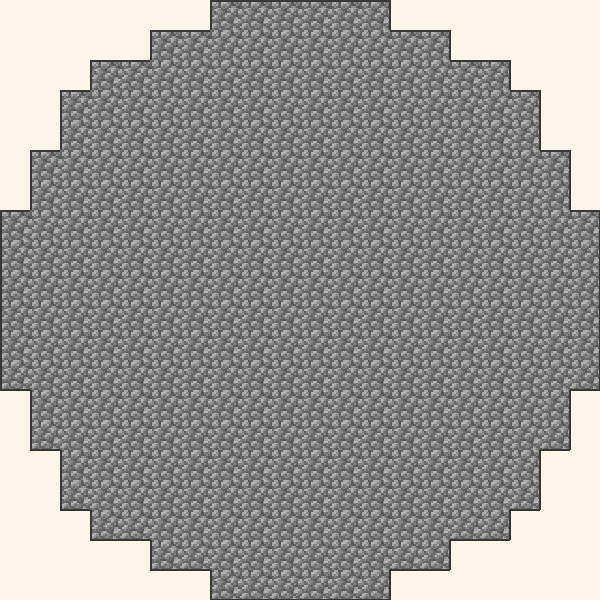
\includegraphics[width=\linewidth]{fig04_2d_d20_euclidean.png}
  \caption{\emph{Euclidien}}
\end{subfigure}\hfill
\begin{subfigure}[t]{0.31\linewidth}\centering
  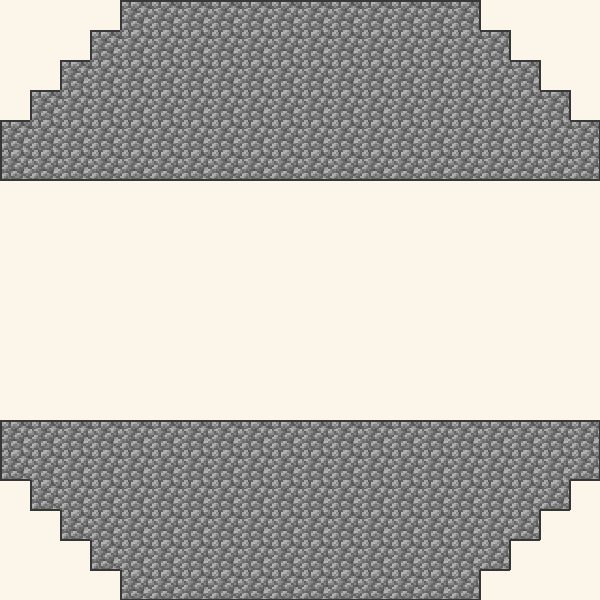
\includegraphics[width=\linewidth]{fig05_2d_d20_bresenham.png}
  \caption{\emph{Bresenham}}
\end{subfigure}\hfill
\begin{subfigure}[t]{0.31\linewidth}\centering
  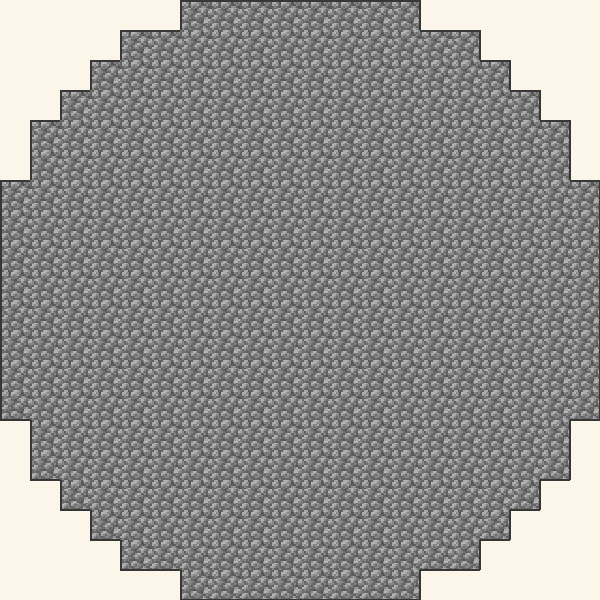
\includegraphics[width=\linewidth]{fig06_2d_d20_threshold.png}
  \caption{\emph{Seuil}}
\end{subfigure}
\caption{Un meme cercle de diametre~20 dans les trois algorithmes, rendu avec la texture cobblestone. L'augmentation du diametre rend les differences plus subtiles --- les trois versions paraissent semblables a l'oeil nu. C'est un bon moment pour commenter que, pour les petits diametres (Figure~\ref{fig:comp-d10}), les differences sont beaucoup plus evidentes.}
\label{fig:comp-d20}
\end{figure}

\begin{minecraft}[Comparaison de blocs : Block Round \emph{vs.} WorldEdit]
A essayer chez soi (si l'on dispose de Minecraft + WorldEdit) : executer \cmd{//sphere stone 10} sur un serveur et compter les blocs. Comparer avec ce que Block Round indique dans l'\emph{Info chip} pour l'algorithme Bresenham, $D = 20$. Les deux comptages doivent coincider (\emph{ou} differer de 0 a 4~blocs en raison de petites differences d'implementation). Si vous trouvez une difference systematique, vous avez decouvert une curiosite mathematique authentique.
\end{minecraft}

% =============================================================================
\subsection{Seance 3 --- \enquote{De l'ellipse a l'ellipsoide : la troisieme dimension}}\label{aula3}

\subsubsection*{Objectif de la seance}
Generaliser l'equation de l'ellipse a l'ellipsoide, introduire les voxels, le calcul de volume discret et les coupes planaires. Etablir des ponts avec le patrimoine architectural francais et avec les constructions celebres de la communaute francophone de Minecraft.

\begin{activite}[3.1 --- De l'equation 2D a la 3D \quad\tempo{15 min}]\label{at:31}
Ajouter une troisieme coordonnee $z$ au repere orthonorme. L'equation implicite de l'ellipse se generalise naturellement :

\begin{formule}
\centering
$\displaystyle \left(\dfrac{x}{r_x}\right)^{\!2} + \left(\dfrac{y}{r_y}\right)^{\!2} + \left(\dfrac{z}{r_z}\right)^{\!2} \;=\; 1$
\end{formule}

Quand $r_x = r_y = r_z = r$, on retrouve la \acc{sphere} $x^2 + y^2 + z^2 = r^2$, comme illustre par la Figure~\ref{fig:3d-shapes}.

\textbf{Voxels :} la cellule d'une grille 3D s'appelle \emph{voxel} (\emph{volume element}). Dans Minecraft, chaque voxel correspond a un \emph{bloc} $1\times1\times1$. Le critere de pertinence est exactement le meme qu'en 2D, augmente de la coordonnee $z$ :

\begin{formule}
\centering
$\displaystyle a_x^2 + a_y^2 + a_z^2 \leq 1,\quad \text{avec } a_\xi = \dfrac{\xi + \tfrac{1}{2} - c_\xi}{r_\xi}$
\end{formule}

\textbf{Demonstration :} ouvrir Block Round en mode 3D, alterner entre Sphere et Ellipsoide, faire tourner avec la \emph{souris}, observer la structure de voxels.
\end{activite}

\begin{figure}[!htbp]
\centering
\begin{subfigure}[t]{0.45\linewidth}\centering
  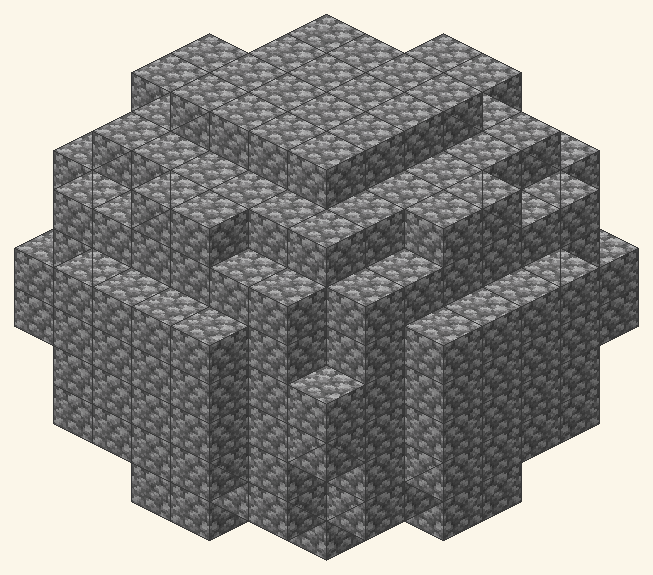
\includegraphics[width=\linewidth]{fig10_3d_sphere_d12.png}
  \caption{Sphere de diametre~10 ($r_x = r_y = r_z = 5$).}
\end{subfigure}\hfill
\begin{subfigure}[t]{0.45\linewidth}\centering
  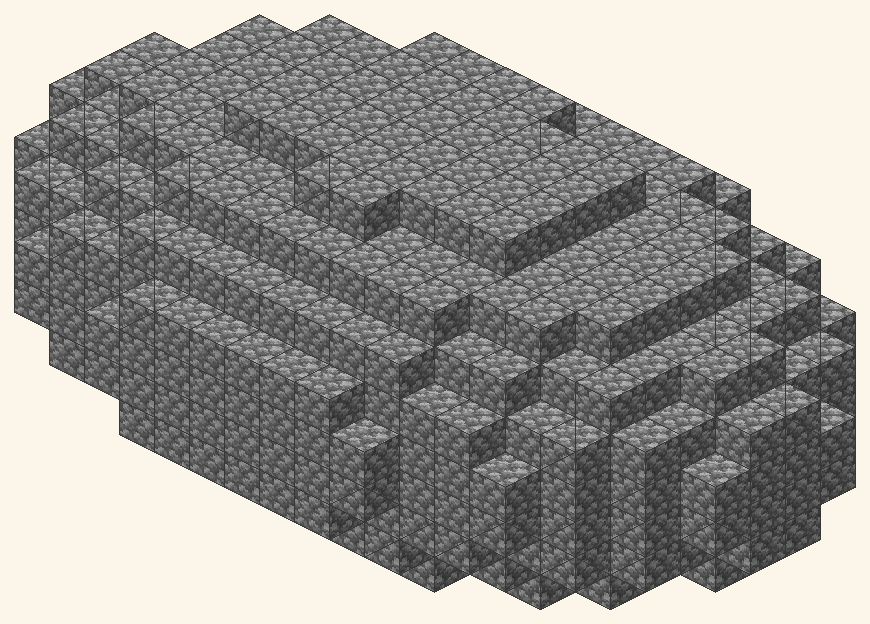
\includegraphics[width=\linewidth]{fig11_3d_ellipsoid.png}
  \caption{Ellipsoide avec $W = 20, H = 10, D = 12$.}
\end{subfigure}
\caption{Voxelisation en 3D. Chaque cube est un voxel (= bloc Minecraft) ; sa coordonnee $(i, j, k)$ au centre est testee dans l'equation implicite. Les escaliers visibles sur la surface sont caracteristiques de la voxelisation --- exactement l'aspect qui donne a Minecraft son identite visuelle.}
\label{fig:3d-shapes}
\end{figure}

\begin{activite}[3.2 --- Volume continu \emph{vs.} discret \quad\tempo{15 min}]\label{at:32}
Le volume continu de l'ellipsoide est un resultat classique :

\begin{formule}
\centering
$\displaystyle V \;=\; \dfrac{4}{3}\,\pi\, r_x\, r_y\, r_z$
\end{formule}

Quand $r_x = r_y = r_z = r$, $V = \tfrac{4}{3}\pi r^3$. Ce contenu est \acc{recurrent au Baccalaureat de specialite Mathematiques} (questions de geometrie spatiale tombees a presque chaque session) et tombe egalement aux \hyperref[sec:olympiades]{Olympiades Academiques de Mathematiques}, en particulier dans les problemes faisant intervenir l'approximation numerique.

\textbf{Activite en binome :}
\begin{enumerate}[leftmargin=1.5em,itemsep=0.15em,topsep=0.3em,nosep]
  \item Calculer le volume continu d'une sphere de diametre 12 ($r = 6$) : $V = \tfrac{4}{3}\pi \cdot 216 \approx 904{,}78$.
  \item Dans Block Round, generer la sphere $D = 12$, mode \emph{Plein}, activer l'\emph{Info chip}, noter le volume discret (nombre de blocs) : environ $V_{\mathrm{disc}} \approx 904$~blocs. \emph{Erreur relative $\approx 0{,}1\%$ --- impressionnante.}
  \item Sur la meme puce, observer la notation \emph{$904 = 14 \times 64 + 8$} : le jeu dira au constructeur en survie \enquote{il vous faut \emph{14 piles completes} de cobblestone + une pile partielle avec \emph{8 blocs}}.
  \item Repeter pour $D = 16$ ($V_{\mathrm{cont}} \approx 2\,144$ ; $V_{\mathrm{disc}} \approx 2\,145$). Noter que pour $D$ pair, l'erreur peut etre \emph{positive} (sur-estimation due au centre entre cellules).
\end{enumerate}

\textbf{Observation :} le rapport $\text{volume discret}/\text{volume continu} \to 1$ quand $D \to \infty$. Pour les petits $D$, il y a une divergence sensible --- et c'est mathematiquement correct : la discretisation \emph{modifie effectivement} le comptage.
\end{activite}

\begin{activite}[3.3 --- Coupes planaires \quad\tempo{10 min}]\label{at:33}
Block Round permet de couper l'ellipsoide par trois plans differents. Chaque coupe est une \acc{inegalite lineaire} appliquee au centre du voxel :

\begin{formule}
\centering
$\begin{array}{lcl}
\text{Axe X :} & x \geq \mathit{cut} & \Rightarrow \text{voxel ecarte} \\
\text{Axe Y :} & y \geq \mathit{cut} & \Rightarrow \text{voxel ecarte} \\
\text{Diagonale :} & x + y \geq \mathit{cut} & \Rightarrow \text{voxel ecarte}
\end{array}$
\end{formule}

La Figure~\ref{fig:cortes} illustre les trois coupes a 50~\%.

\textbf{Discussion dirigee :} \emph{\enquote{Pourquoi une coupe diagonale a-t-elle une amplitude $D_x + D_y$ et non $D_x$ ? Ou se trouve l'hypotenuse ?}} Conduire a reconnaitre que $x + y$ prend des valeurs entre $0$ et $D_x + D_y$ dans la boite rectangulaire. \emph{Dans Minecraft, une coupe Y a 50~\% sur une sphere produit une \enquote{coupole} classique --- la moitie superieure de la sphere, qui est exactement la construction qui couvre temples, observatoires et arenes sur des milliers de serveurs.}
\end{activite}

\begin{figure}[!htbp]
\centering
\begin{subfigure}[t]{0.31\linewidth}\centering
  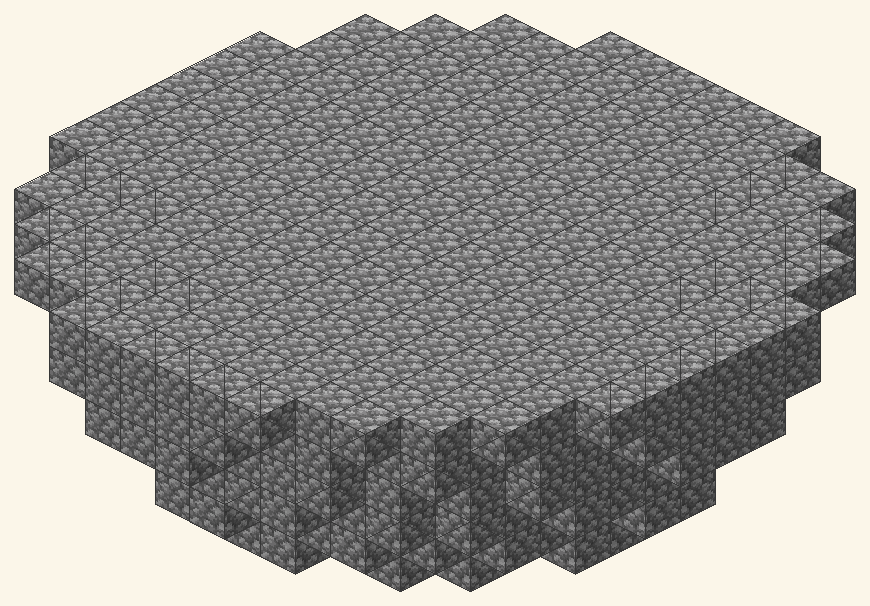
\includegraphics[width=\linewidth]{fig12_3d_cut_y50.png}
  \caption{Coupe Y a 50~\% --- la \emph{coupole} classique.}
\end{subfigure}\hfill
\begin{subfigure}[t]{0.31\linewidth}\centering
  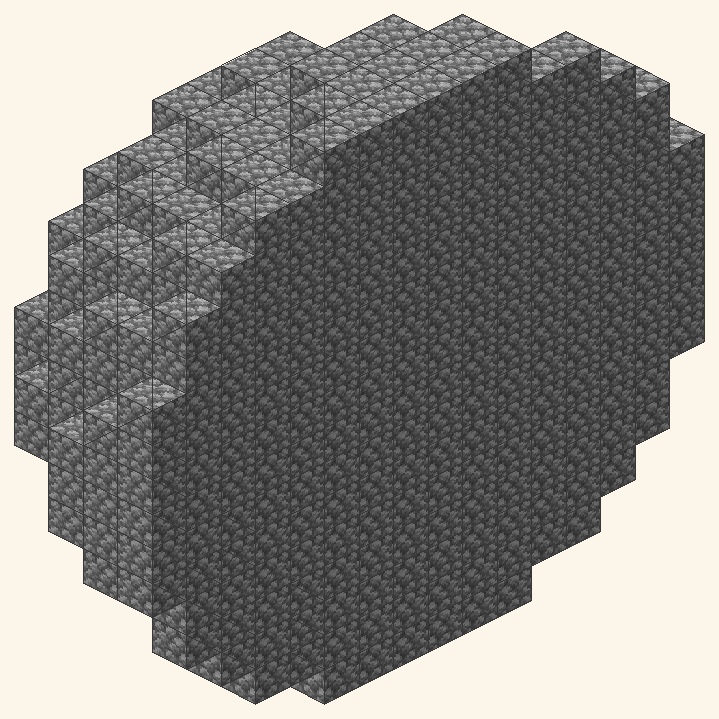
\includegraphics[width=\linewidth]{fig13_3d_cut_x50.png}
  \caption{Coupe X a 50~\% --- une \emph{demi-sphere laterale}.}
\end{subfigure}\hfill
\begin{subfigure}[t]{0.31\linewidth}\centering
  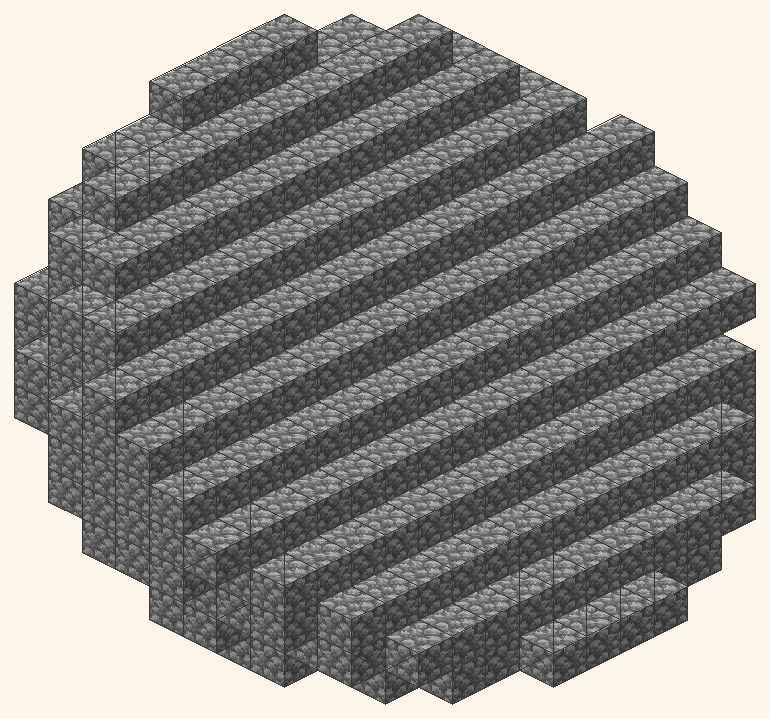
\includegraphics[width=\linewidth]{fig14_3d_cut_diag50.png}
  \caption{Coupe diagonale a 50~\% --- une \emph{demi-cuvette} oblique.}
\end{subfigure}
\caption{Trois coupes planaires sur le meme ellipsoide de diametre 16, toutes conservant 50~\% du volume. Observez le motif en escalier caracteristique de la coupe diagonale : il revele l'hypotenuse qui relie les deux axes. Chaque coupe est un plan de construction Minecraft different : coupole de temple, demi-arene laterale, amphitheatre de fontaine.}
\label{fig:cortes}
\end{figure}

\begin{activite}[3.4 --- Dialogue avec le patrimoine architectural francais \quad\tempo{10 min}]\label{at:34}
\emph{Connexion avec Arts plastiques, Histoire et Histoire des Arts. Cette activite met en oeuvre les competences du programme sur identite culturelle et patrimoine.}

Projeter (ou distribuer en version imprimee) cinq images :

\begin{itemize}[leftmargin=1.3em,itemsep=0.2em,topsep=0.3em,nosep]
  \item \acc{Notre-Dame du Haut, Ronchamp} (Le Corbusier, 1955) : ses toits courbes en beton arme constituent un assemblage de \emph{paraboloides hyperboliques} construit a la regle et au compas, puis coule. Avec la \emph{Villa Savoye} (Poissy) et l'\emph{Unite d'Habitation de Marseille}, Le Corbusier a realise a l'echelle architecturale les memes courbes que celles que nous etudions. Le \emph{Centre Pompidou} (Piano, Rogers, Paris, 1977) montre une grille modulaire visible --- presque voxelisee --- a l'echelle d'un musee.

  \item \acc{Fondation Louis Vuitton} (Frank Gehry, Paris, 2014) : voiles courbes en verre dont la generation algorithmique repose sur la voxelisation de surfaces de Bezier. Le \emph{Pavillon Soulages} (RCR Arquitectes, Rodez) est un autre exemple contemporain. La Pyramide du Louvre (I.M. Pei, 1989) propose au contraire une geometrie pure : tetraedres de verre, sphere et pyramide en dialogue.

  \item \acc{Bories du Vaucluse et bergeries des Cevennes} : les architectures vernaculaires en pierre seche illustrent la \emph{construction par voxels manuels}. Chaque pierre est un \enquote{bloc} pose en respectant des regles d'encorbellement qui rappellent les algorithmes de Bresenham : le tailleur de pierre place ses pierres en suivant un critere geometrique transmis oralement. Tradition mathematique vivante, anterieure a l'ordinateur.

  \item \acc{Vitraux gothiques de Chartres et de la Sainte-Chapelle} : les rosaces et vitraux de Notre-Dame de Paris (avant l'incendie de 2019), de Chartres et de la Sainte-Chapelle constituent une \emph{tessellation \enquote{voxel en verre}} d'une sophistication geometrique remarquable. Les motifs preferent souvent des pavages decoratifs proches des \emph{tessellations de Penrose} (avant l'heure !). La \emph{Tapisserie de Bayeux} (XIe~siecle), elle, est une \emph{rasterisation textile} : chaque maille de laine est un \enquote{pixel}, le motif est une frise discretisee.

  \item \acc{Constructions de la communaute francophone Minecraft} : cites construites sur des serveurs comme \emph{ProtagonyX}, \emph{Funcraft}, \emph{Hypixel} francais, ou sur les serveurs scolaires. On peut montrer des \emph{timelapses} de constructions de coupoles, spheres et arcs publies sur YouTube francophone (Aypierre, Inoxtag, Frigiel \& Fluffy, Siphano). \emph{C'est la praxeologie francophone Minecraft en action}, contemporaine, vivante, en francais.
\end{itemize}

\textbf{Discussion dirigee :} \emph{\enquote{Le Corbusier a projete dans le beton les memes courbes que vous avez dessinees avec des blocs. Les batisseurs des bories du Vaucluse ont resolu, avec leurs mains, le probleme de la voxelisation des coupoles bien avant l'invention des ordinateurs. Les vitraux de Chartres dessinent des cercles en verre depuis huit siecles. La communaute francophone Minecraft fait la meme chose en direct, tous les jours, sur des serveurs partages. Le probleme de la rasterisation que nous etudions n'est pas une invention de l'ere numerique : c'est une constante de l'histoire humaine. Chaque culture a trouve sa maniere de \emph{rasteriser}.}}

\textbf{Articulation interdisciplinaire :} partenariat suggere avec l'enseignant\textperiodcentered e d'Arts plastiques, d'Histoire-Geographie et/ou d'Histoire des Arts pour approfondissement. Les Seances~\ref{aula4} et~\ref{aula5} peuvent demander aux groupes de \emph{choisir} quelle tradition visuelle francaise inspirera leur travail.
\end{activite}

% =============================================================================
\subsection{Seance 4 --- \enquote{Arithmetique de l'inventaire : piles, coffres, commandes}}\label{aula4}

\subsubsection*{Objectif de la seance}
Introduire l'\emph{arithmetique d'inventaire} de Minecraft comme application concrete de la division avec plafond et de la representation quotient-reste. Presenter les commandes centrales (\cmd{/fill}, \cmd{/clone}, \cmd{//sphere}, \cmd{//hsphere}) et l'optimisation par symetrie octaedrique.

\begin{activite}[4.1 --- Arithmetique des piles \quad\tempo{15 min}]\label{at:41}
Dans Minecraft, chaque emplacement de l'inventaire contient au maximum \acc{64 blocs identiques}. Cette limite donne sens pratique au calcul de volume : $V = 904$~blocs pour une sphere $D=12$ ne signifie \emph{pas} \enquote{904 dans la besace} --- cela signifie \enquote{$\lceil 904/64 \rceil = 15$~piles (emplacements pleins)} de cobblestone.

\textbf{Formules cles :}

\begin{formule}
\centering
$\displaystyle N_{\mathrm{piles}} = \left\lceil \dfrac{V}{64} \right\rceil
\qquad\qquad
N_{\mathrm{coffres\,doubles}} = \left\lceil \dfrac{V}{3\,456} \right\rceil$
\end{formule}

(Un coffre simple a 27~emplacements ; un coffre double, 54~emplacements ; $54 \times 64 = 3\,456$ articles par coffre double.)

\textbf{Activite en binome :}
\begin{enumerate}[leftmargin=1.5em,itemsep=0.15em,topsep=0.3em,nosep]
  \item Pour une sphere $D = 8$ (volume $\approx 268$~blocs) : combien de piles ? Combien de coffres simples ? Reponse : 5~piles ; 1~coffre simple (avec 17~emplacements libres).
  \item Pour une sphere $D = 16$ (volume $\approx 2\,145$~blocs) : combien de piles ? Combien de coffres doubles ? Reponse : 34~piles ; 1~coffre double (il manque 20~piles pour le remplir --- il reste donc de la place pour un autre petit cylindre).
  \item Pour une sphere $D = 32$ (volume $\approx 17\,156$~blocs) : combien de piles ? Combien de coffres doubles ? Reponse : 269~piles (soit environ 5~coffres doubles + 1~pile), $\lceil 17\,156/3\,456 \rceil = 5$~coffres doubles.
  \item \emph{Dans Minecraft, en mode survie, un mineur francophone extrait typiquement 1~pile de cobblestone toutes les 4 a 6~minutes (selon la pioche). Calculer le temps total estime de collecte pour la sphere $D = 16$ : $34 \times 5 = 170$~minutes $\approx 2{,}8$~heures.}
\end{enumerate}
\end{activite}

\begin{activite}[4.2 --- Commandes Minecraft \quad\tempo{15 min}]\label{at:42}
Presenter les commandes centrales :

\begin{itemize}[leftmargin=1.4em,itemsep=0.25em,topsep=0.3em]
  \item \cmd{/setblock x y z minecraft:stone} --- place un bloc a une position specifique.
  \item \cmd{/fill x1 y1 z1 x2 y2 z2 minecraft:stone} --- remplit une boite rectangulaire avec un bloc. Limite vanilla : 32\,768~blocs par commande.
  \item \cmd{/clone x1 y1 z1 x2 y2 z2 x3 y3 z3} --- copie une region vers une autre position (pouvoir fondamental pour la construction par symetrie).
  \item \cmd{//sphere stone 8} (WorldEdit) --- dessine une sphere de rayon 8 centree sur le joueur, avec l'algorithme Bresenham 3D.
  \item \cmd{//hsphere stone 8} (WorldEdit) --- dessine une sphere \emph{creuse} (uniquement la coque). Utile pour les coupoles vides a l'interieur.
  \item \cmd{//ellipsoid stone 10 5 10} (WorldEdit) --- ellipsoide $W = 20, H = 10, D = 20$ avec demi-axes specifies.
\end{itemize}

\textbf{Demonstration (si Minecraft est disponible) :} executer \cmd{//sphere stone 8} dans un monde de test et chronometrer. Comparer avec ce que Block Round affiche pour diametre 16, algorithme Bresenham. Confirmer l'identite mathematique des deux sorties.

\textbf{Si Minecraft n'est pas disponible :} executer mentalement. Noter sur papier quadrille : \enquote{Je suis au sol (y=64). Je veux une sphere de rayon 8 a partir de y=72 (8~blocs au-dessus du sol). Quelle commande ?} Reponse : \cmd{//sphere stone 8} en se positionnant a $(0, 72, 0)$.
\end{activite}

\begin{activite}[4.3 --- Optimisation par symetrie octaedrique \quad\tempo{15 min}]\label{at:43}
\textbf{Idee centrale :} une sphere centree en l'origine est invariante par reflexions dans les trois plans de coordonnees. Le groupe $\mathbb{Z}_2^3$ a pour ordre 8 : a partir d'un \emph{octant} (region $+x, +y, +z$), les sept autres regions s'obtiennent par reflexion.

\textbf{Implication pratique :} au lieu de poser $V$~blocs un a un, construire $V/8$~blocs dans l'octant positif et refleter 7~fois avec \cmd{/clone}.

\begin{formule}
\centering
$\displaystyle \mathrm{cout}_\mathrm{symetrie} = N_\mathrm{octant} + 7\, T_\mathrm{clone}
\;\ll\; \mathrm{cout}_\mathrm{force\,brute} = N\, T_\mathrm{bloc}$
\end{formule}

\textbf{Exemple concret, sphere $D = 24$ centree en $(0, 72, 0)$ :}
\begin{enumerate}[leftmargin=1.5em,itemsep=0.15em,topsep=0.3em,nosep]
  \item Construire manuellement l'octant positif ($\approx 905$~blocs, $\approx 15$~minutes en survie ou $\approx 45$~secondes en creatif avec brush).
  \item Refleter en $-x$ : \cmd{/clone 0 72 0 12 84 12 -12 72 0 mode:masked}
  \item Refleter en $-y$ : \cmd{/clone 0 72 0 12 84 12 0 60 0 mode:masked}
  \item Refleter en $-z$ : \cmd{/clone 0 72 0 12 84 12 0 72 -12 mode:masked}
  \item Octants $(-x, -y)$, $(-y, -z)$, $(-x, -z)$, $(-x, -y, -z)$ : commandes analogues.
\end{enumerate}

\textbf{Comparaison de temps :}
\begin{itemize}[leftmargin=1.3em,itemsep=0.1em,topsep=0.2em,nosep]
  \item Sans symetrie, en survie : 7\,238~blocs $\times$ 2~s/bloc $\approx$ 4~heures.
  \item Avec symetrie : 15~min (octant) + 0{,}5~s (7~clones) $\approx$ 15~min.
  \item Acceleration : \emph{facteur 16}.
\end{itemize}
\end{activite}

\begin{activite}[4.4 --- Application : planifier une coupole reelle \quad\tempo{5 min}]
En binome, planifier (\emph{sur papier ou sur Block Round}) la construction d'une coupole en Quartz $D=20$ au sommet d'un temple stylise inspire de Le Corbusier, des bories provencales ou des cases creoles. Noter :
\begin{itemize}[leftmargin=1.3em,itemsep=0.1em,topsep=0.2em,nosep]
  \item Volume de la coupole (moitie de la sphere $D=20$) : $\approx 2\,094$~blocs.
  \item Piles necessaires : 33~piles.
  \item Nombre de Quartz blocks (chacun exige 4~Nether Quartz, minerables dans le Nether) : $\sim 2\,094 \times 4 = 8\,376$~Nether Quartz.
  \item Sequence de commandes optimisee par symetrie.
\end{itemize}

Cette activite prepare le terrain pour la Seance~5 (construction reelle).
\end{activite}

% =============================================================================
\subsection{Seance 5 --- \enquote{Construction reelle : de Block Round a Minecraft}}\label{aula5}

\subsubsection*{Objectif de la seance}
Mobiliser l'ensemble du contenu developpe en un \emph{produit auctorial construit} : exporter depuis Block Round, importer dans Minecraft (via Litematica ou Schematica), executer la construction en creatif ou en survie. Evaluer les apprentissages par la defense argumentative des choix mathematiques et la remise du produit final.

\begin{activite}[5.1 --- Presentation du defi \quad\tempo{5 min}]\label{at:51}
\textbf{Consigne :} \emph{\enquote{En binomes ou trinomes, vous allez produire une construction dans Minecraft (ou sur Block Round, si Minecraft n'est pas disponible) qui combine au moins trois figures generees par Block Round (cercles, ellipses, spheres ou ellipsoides). Cela peut etre une cite sur le serveur de la classe, un temple, une ferme circulaire, un observatoire --- vous choisissez. A la fin, chaque groupe presentera son oeuvre en expliquant \acc{mathematiquement} ses choix : pourquoi cet algorithme ? pourquoi cette proportion ? pourquoi cette coupe ? pourquoi ces blocs ?}}
\end{activite}

\begin{activite}[5.2 --- Exportation et importation \quad\tempo{15 min}]\label{at:52}
Demontrer le flux Block Round $\rightarrow$ Minecraft :

\begin{enumerate}[leftmargin=1.5em,itemsep=0.2em,topsep=0.3em]
  \item Sur Block Round, configurer la figure souhaitee (par exemple : sphere $D = 12$ en Quartz avec coupe Y a 50~\%).
  \item Cliquer sur le bouton \emph{Export Schematic} dans le coin du canvas. Le fichier \texttt{.schem} (Sponge Schematic v2) est telecharge.
  \item Dans Minecraft Java Edition avec le mod \emph{Litematica} installe (gratuit) : ouvrir le mod, \emph{Load Schematic}, selectionner le fichier telecharge.
  \item Litematica affiche un \enquote{fantome} translucide de la construction a la position choisie par le joueur.
  \item Le joueur place chaque bloc \emph{en suivant le fantome}. Litematica met en rouge tout bloc mal place.
  \item \emph{Alternative via \cmd{//schem load} :} sur serveur avec WorldEdit, \cmd{//schem load nom\_fichier} importe le schematic, et \cmd{//paste -a} colle a la position courante --- construction instantanee.
\end{enumerate}

\textbf{Si Minecraft n'est pas disponible :} demontrer l'exportation du \texttt{.schem} et afficher le fichier binaire avec un editeur hexadecimal --- discussion sur le format Sponge v2, gzip, NBT. Itineraire formatif vers la specialite NSI.
\end{activite}

\begin{activite}[5.3 --- Production \quad\tempo{20 min}]\label{at:53}
\textbf{Materiel par groupe :}
\begin{itemize}[leftmargin=1.3em,itemsep=0.15em,topsep=0.3em,nosep]
  \item Acces a Block Round (ordinateur ou \emph{smartphone}) ;
  \item (Optionnel) Acces a Minecraft avec Litematica ou Schematica ;
  \item Papier quadrille, crayons et feutres pour esquisses et plan ;
  \item Fiche-plan avec trois questions obligatoires (Annexe~\ref{ap:exerc}, exercice 8).
\end{itemize}

\textbf{Etapes internes du travail de groupe :}
\begin{enumerate}[leftmargin=1.5em,itemsep=0.15em,topsep=0.3em,nosep]
  \item \tempo{5 min} Brainstorming et esquisse sur papier.
  \item \tempo{8 min} Production sur Block Round et exportation du \texttt{.schem}.
  \item \tempo{5 min} Importation dans Minecraft et test rapide (si disponible).
  \item \tempo{2 min} Redaction de la justification mathematique sur la fiche.
\end{enumerate}

\textbf{Accompagnement de l'enseignant\textperiodcentered e :} circuler entre les groupes, en posant des questions mediatrices --- \emph{\enquote{Pourquoi avez-vous choisi cet algorithme ? Comment cette coupe pourrait-elle s'ecrire comme une inegalite ? Combien de coffres doubles de Quartz vous faudra-t-il ?}}
\end{activite}

\begin{activite}[5.4 --- Presentation et synthese collective \quad\tempo{10 min}]\label{at:54}
Chaque groupe dispose de 2~minutes pour presenter son oeuvre a la classe, en la projetant (ou sur Minecraft, ou physiquement sur papier) et en repondant a \emph{au moins une} des trois questions mathematiques exigees.

\textbf{Criteres minimaux de la presentation :}
\begin{itemize}[leftmargin=1.3em,itemsep=0.1em,topsep=0.2em,nosep]
  \item identifier au moins une figure mathematique presente ;
  \item nommer l'algorithme choisi et justifier (meme \emph{a posteriori}) pourquoi il convient a l'effet visuel vise ;
  \item s'il y a une coupe 3D, la decrire comme une inegalite ;
  \item estimer (meme grossierement) le nombre de piles / coffres necessaires.
\end{itemize}

\textbf{Synthese finale par l'enseignant\textperiodcentered e (3~min) :} reprendre l'idee centrale de la sequence --- \emph{\enquote{sur une grille discrete de voxels, une meme courbe continue admet plusieurs representations ; en choisir une est une decision mathematique ; la construire dans Minecraft est une decision de citoyennete, de gestion de ressources et d'esthetique}} --- et la situer dans l'horizon de la mathematique francaise contemporaine : inviter la classe a explorer les \hyperref[sec:olympiades]{Olympiades Academiques de Mathematiques}, a en savoir plus sur Hugo Duminil-Copin et Cedric Villani, et a participer a des serveurs Minecraft francophones qui encouragent les constructions collaboratives.
\end{activite}

\begin{minecraft}[Pistes de prolongement]
Cette Seance~5 ouvre plusieurs pistes de prolongement en projet extra-scolaire :
\begin{itemize}[leftmargin=1.3em,itemsep=0.15em,topsep=0.3em,nosep]
  \item \textbf{Projet \enquote{Cite Mathematique} :} la classe construit une cite sur le serveur du lycee, ou chaque batiment realise une figure geometrique (cylindre, sphere, ellipsoide, jeu de coniques).
  \item \textbf{Reconstitution du patrimoine francais :} reconstruction dans Minecraft de Notre-Dame du Haut (Ronchamp), de la Tour Eiffel, de la Pyramide du Louvre, de la Fondation Louis Vuitton, du Pont du Gard, ou d'une borie provencale.
  \item \textbf{Olympiade Block Round :} competition interne --- qui construit la sphere la plus proche du volume continu ? qui optimise le mieux le temps grace a la symetrie ?
  \item \textbf{Articulation avec les Sciences de l'ingenieur :} utiliser Block Round comme bac a sable de pre-ingenierie : coupoles geodesiques, treillis voxelises, structures qui approchent des surfaces lisses --- preparation aux ecoles d'ingenieurs (Polytechnique, Centrale, Mines, Ponts).
  \item \textbf{Articulation avec NSI :} reimplementer les trois algorithmes en Python ou Scratch, comparer les sorties avec Block Round, soumettre l'analyse comme projet pour le Grand Oral.
\end{itemize}
\end{minecraft}


% =============================================================================
\section{Evaluation}\label{sec:avaliacao}

L'evaluation adopte un modele \acc{formatif}, \acc{processuel} et \acc{sommatif}, articulant quatre dimensions (plus une dimension specifique a l'application dans Minecraft) et dialoguant avec la tradition francaise de l'evaluation par competences (Meirieu, 2004 ; Perrenoud, 1997).

\subsection{Evaluation diagnostique}
Realisee en Seance~\ref{aula1}, au moment de l'Activite~1.2 (dessin manuel du cercle). Elle permet a l'enseignant\textperiodcentered e d'identifier les difficultes avec le repere orthonorme, l'equation du cercle et le comptage --- et de combler les lacunes post-pandemiques attestees par les evaluations DEPP entre 2021 et 2024.

\subsection{Evaluation formative}
Distribuee sur les cinq seances : observation directe de la participation, qualite des reponses dans le \emph{think--pair--share}, correction \emph{immediate} des calculs des Activites~\ref{at:25}, \ref{at:32} et~\ref{at:41}.

\subsection{Evaluation sommative}
Composee de deux livrables :

\begin{enumerate}[leftmargin=1.5em,itemsep=0.2em,topsep=0.3em,nosep]
  \item \textbf{Liste d'exercices} (Annexe~\ref{ap:exerc}), 8~questions, remise a la fin de la Seance~\ref{aula5} ou a une date convenue.
  \item \textbf{Projet final} (Activite~\ref{at:53}), accompagne d'une fiche-plan remplie pour la defense (Activite~\ref{at:54}).
\end{enumerate}

\subsection{Grille d'evaluation}

\begin{center}
\small
\begin{tabularx}{\textwidth}{@{}p{0.21\textwidth}XX@{}}
\toprule
\textbf{Dimension} & \textbf{Pleinement satisfaisant (8--10)} & \textbf{Partiellement satisfaisant (5--7) / Insuffisant (0--4)} \\
\midrule
\textbf{Concepts mathematiques} & Applique correctement l'equation implicite de l'ellipse/ellipsoide ; reconnait les trois criteres algorithmiques et leurs differences. & Applique l'equation de base du cercle mais peine sur la generalisation a l'ellipse / ne reconnait pas les differences algorithmiques. \\
\addlinespace[3pt]
\textbf{Usage du logiciel (Block Round)} & Opere Block Round avec autonomie en 2D et 3D ; exporte images et \texttt{.schem} ; alterne algorithmes et styles. & A besoin d'aide frequente ; n'opere qu'en 2D. \\
\addlinespace[3pt]
\textbf{Argumentation} & Justifie mathematiquement ses choix dans le projet final ; emploie un vocabulaire technique approprie (\emph{algorithme}, \emph{voxel}, \emph{coupe}, \emph{inegalite}, \emph{pile}, \emph{coffre double}). & Justifie esthetiquement, sans mobiliser les mathematiques ; vocabulaire absent. \\
\addlinespace[3pt]
\textbf{Application pratique Minecraft} & Calcule correctement piles et coffres pour le projet ; decrit la sequence de commandes \cmd{/fill} ou \cmd{//sphere} ; utilise la symetrie octaedrique. & Confond quotient et reste ; traite les blocs comme des unites isolees ; n'utilise pas la symetrie. \\
\addlinespace[3pt]
\textbf{Cooperation} & Travaille productivement en binome / trinome ; contribue a la discussion collective. & Travaille isolement ; peu de contribution. \\
\bottomrule
\end{tabularx}
\end{center}

\subsection{Conversion en notes}
\begin{itemize}[leftmargin=1.3em,itemsep=0.1em,topsep=0.2em,nosep]
  \item Liste d'exercices : 40~\% de la note.
  \item Projet final + presentation : 50~\% de la note.
  \item Observation processuelle (participation) : 10~\% de la note.
\end{itemize}

% =============================================================================
\section{Articulations avec l'ecosysteme mathematique francais}\label{sec:olympiades}

La sequence s'inscrit dans un \emph{ecosysteme riche} d'initiatives francaises d'enseignement et de recherche en mathematiques et en technologie, que l'enseignant\textperiodcentered e peut mobiliser comme prolongement ou approfondissement.

\subsection{Olympiades Academiques de Mathematiques}

Les \href{https://eduscol.education.fr/}{Olympiades Academiques de Mathematiques} ont lieu chaque annee depuis 2001 en classe de Premiere (et depuis 2005 en Terminale), organisees par les rectorats d'academie avec le soutien de l'Inspection Generale et l'Association \emph{Animath}. Elles se deroulent en mars et primez les meilleurs eleves par academie. \emph{Le contenu de cette sequence (geometrie reperee du cercle et de l'ellipsoide, raisonnement algorithmique, approximations numeriques) prepare directement aux exercices de l'epreuve.}

\subsection{Olympiades Francaises de Mathematiques (OFM)}

Les \href{https://www.animath.fr/}{Olympiades Francaises de Mathematiques}, animees par \emph{Animath} et l'UMPA (ENS de Lyon), selectionnent l'equipe nationale francaise pour l'\emph{Olympiade Internationale de Mathematiques} (IMO). Stages Maths C Pour Tous, stage olympique d'Animath, POFM (\emph{Pole Olympique Francais de Mathematiques}). Cette sequence peut etre \emph{porte d'entree} : les eleves qui se distinguent au projet final de la Seance~\ref{aula5} peuvent etre encourages a participer a l'edition suivante.

\subsection{Hugo Duminil-Copin et l'IHES}

En 2022, \acc{Hugo Duminil-Copin} (ne en 1985, IHES Bures-sur-Yvette et Universite de Geneve) est devenu, a 36~ans, l'un des plus jeunes Francais a recevoir la \emph{Medaille Fields} --- la plus haute distinction des mathematiques mondiales. Avant lui : Cedric Villani (2010), Wendelin Werner (2006), Laurent Lafforgue (2002), Pierre-Louis Lions (1994). Tous ces mathematiciens francais sont rattaches a l'\href{https://www.ihes.fr/}{IHES} (Institut des Hautes Etudes Scientifiques, Bures-sur-Yvette, modele inspire de Princeton IAS) et au CNRS (sections INSMI), avec collaborations avec l'INRIA, l'Institut Henri Poincare (IHP, Paris) et le CIRM (Centre International de Rencontres Mathematiques, Marseille).

La tradition mathematique francaise est ancienne : \emph{Henri Poincare} (1854--1912, topologie, conjecture de Poincare resolue par Perelman en 2002), \emph{Sophie Germain} (1776--1831, premiere femme membre associee de l'Academie des Sciences, theorie des nombres et elasticite), \emph{Evariste Galois} (1811--1832, theorie des groupes, mort prematurement a 20~ans), \emph{Alexander Grothendieck} (Medaille Fields 1966, theorie des schemas, fondateur de la modernite mathematique francaise).

\subsection{France-IOI, Castor Informatique, Alkindi}

Les concours d'informatique pour lyceens sont nombreux en France : \href{https://www.france-ioi.org/}{France-IOI} (entrainement aux Olympiades Internationales d'Informatique) ; \href{https://castor-informatique.fr/}{Concours Castor Informatique} (chaque automne, plus de 700\,000 participants) ; \href{https://www.concours-alkindi.fr/}{Concours Alkindi} (cryptographie, classes de Quatrieme a Seconde). L'algorithme de Bresenham (traite en Activite~\ref{at:23}) est un theme classique de ces concours.

\subsection{Concours Kangourou des Mathematiques}

Le \href{https://www.mathkang.org/}{Concours Kangourou} (chaque annee en mars, plus de 250\,000 participants en France) propose des QCM ouverts aux classes de la maternelle au lycee. Tradition francaise importante de mathematiques recreatives, dans la ligne de Martin Gardner et de la \emph{Federation Francaise des Jeux Mathematiques}.

\subsection{Minecraft Education (Microsoft Education et Reseau Canope)}\label{sec:mee}

\emph{Minecraft Education} est disponible via l'offre \emph{Microsoft~365 Education} (gratuite pour les enseignants verifies avec une adresse academique \texttt{prenom.nom@ac-XXX.fr}). Le \href{https://www.reseau-canope.fr/}{Reseau Canope} propose des formations et des ressources en francais. Plusieurs academies (Paris, Lyon, Versailles, Aix-Marseille) ont signe des accords-cadres avec Microsoft Education. \emph{Cette sequence est compatible} : le \texttt{.schem} exporte par Block Round peut etre importe dans Java Edition (via Litematica) ou adapte pour Education (via cmdblocks ou import indirect).

\subsection{Communautes francophones d'arcade et d'architecture voxel}

La communaute francophone Minecraft compte des chaines specialisees en \emph{redstone engineering} (logique computationnelle implementee avec des circuits dans le jeu --- equivalent des circuits numeriques reels) et en \emph{megaconstructions architecturales}. Aypierre (serie historique \emph{Aventure}), Frigiel \& Fluffy (fictions Minecraft), Siphano (commentateur d'aventures), Inoxtag (createur tres suivi, projet Everest), TonTon (Quebec francophone) sont des references culturelles que l'enseignant\textperiodcentered e peut mobiliser pour la contextualisation. \emph{Activite complementaire :} demander aux eleves d'apporter un lien vers un tutoriel en francais et d'analyser la mathematique implicite.

\subsection{Ethnomathematique (D'Ambrosio) et didactique francaise (Brousseau, Chevallard)}

La ligne de recherche en ethnomathematique, fondee par le bresilien \acc{Ubiratan D'Ambrosio} (1932--2021), a recu l'ICMI Felix Klein Award (2005) --- distinction mondiale en education mathematique. Bibliographie initiale : D'Ambrosio (traduit au CNRS), \emph{Ethnomathematique : entre tradition et modernite}. Du cote francais : Guy Brousseau (TSD), Yves Chevallard (TAD), Regine Douady (jeu de cadres) et l'ecole de l'IREM (Institut de Recherche sur l'Enseignement des Mathematiques) dans chaque academie.

\subsection{Formation continue : CAPES, Agregation, M2 MEEF, IREM}

Le \href{https://www.devenirenseignant.gouv.fr/}{CAPES de Mathematiques} et l'\href{https://www.devenirenseignant.gouv.fr/}{Agregation de Mathematiques} sont les concours de recrutement des enseignant\textperiodcentered es du secondaire. Le \emph{M2 MEEF} (Metiers de l'Enseignement, de l'Education et de la Formation) est le master qui prepare a ces concours. La formation continue passe par le \emph{Plan National de Formation} (PNF) du Ministere de l'Education nationale, par les \emph{IREM} (Instituts de Recherche sur l'Enseignement des Mathematiques) presents dans chaque academie, et par les actions de Reseau Canope. Cette sequence peut servir de base a un memoire de M2 MEEF ou a une action de formation IREM.

% =============================================================================
\section{Articulations interdisciplinaires}\label{sec:interdisc}

\subsection{Avec les Arts plastiques}
La production de \emph{voxel art} est traditionnellement abordee comme langage artistique. Block Round offre une rare occasion d'articuler Mathematiques et Arts sous un meme objet : la figure \emph{est simultanement} une equation et une composition esthetique. Suggestion : partenariat avec l'enseignant\textperiodcentered e d'Arts plastiques pour une exposition finale des travaux sur le mur ou les reseaux sociaux du lycee. Approfondissement possible : etude des artistes francais geometriques --- Sonia Delaunay (Orphisme), Auguste Herbin (cubisme tardif geometrique), Victor Vasarely (Op art, voxelisation en peinture, Fondation Vasarely a Aix-en-Provence), Yves Klein (monochromes IKB, voxels conceptuels), Daniel Buren (rayures modulaires), Niki de Saint Phalle (Fontaine Stravinsky a Paris).

\subsection{Avec la Physique-Chimie}
La couche sonore de Block Round utilise une synthese additive d'ondes sinusoidales (similaire a Pixel Round). Les frequences choisies approchent les notes du \acc{temperament egal a 12~sons} (chaque demi-ton multiplie la frequence par $2^{1/12} \approx 1{,}0595$). Contenu articule avec \emph{Ondes mecaniques}, \emph{Acoustique} et \emph{Fonctions exponentielles}. Tradition francaise : Jean-Philippe Rameau (\emph{Traite de l'harmonie}, 1722, fondement theorique du temperament egal) ; Pierre Boulez et l'IRCAM (Institut de Recherche et Coordination Acoustique/Musique, Paris, Centre Pompidou). Dans Minecraft, articulation avec la \emph{redstone} (logique numerique), les blocs de note (notes musicales), la simulation physique (chute du sable, ecoulement de l'eau).

\subsection{Avec la specialite NSI (Numerique et Sciences Informatiques)}
L'algorithme de Bresenham est une reference classique de l'informatique. Articuler avec les cours de \emph{pensee computationnelle} de la specialite NSI : \emph{abstraction} (l'equation comme modele), \emph{decomposition} (la forme comme ensemble de voxels), \emph{reconnaissance de motifs} (symetries), \emph{algorithmique} (les trois procedures). Connexion directe avec le programme NSI de Premiere et Terminale, avec les concours France-IOI et Castor Informatique. La generation du \texttt{.schem} (format Sponge v2 avec gzip + NBT) est un \emph{cas d'etude} de serialisation binaire --- programme de la specialite NSI en Terminale, partie \emph{Donnees structurees}. Reference incontournable : Claude Shannon (theorie de l'information, 1948) et le programme INRIA \emph{Pixees} (\url{https://pixees.fr/}).

\subsection{Avec l'Histoire et l'Histoire des Arts}
Bresenham a publie l'algorithme en 1965, en plein apogee de l'informatique \emph{mainframe} chez IBM. Au meme moment, la France lancait le \emph{Plan Calcul} (1966, sous l'impulsion du general de Gaulle), qui mena a la creation de la \emph{CII} (Compagnie Internationale pour l'Informatique) puis de l'\emph{IRIA} (1967, ancetre de l'\href{https://www.inria.fr/}{INRIA}). Plus tot encore : \emph{Blaise Pascal} (Pascaline, 1645, premiere machine a calculer mecanique au monde, precurseur francais !) ; \emph{Bouchon et Falcon} (cartes perforees textiles a Lyon vers 1725, precurseurs de la programmation, reconnus par Jacquard en 1801) ; \emph{Jacques de Vaucanson} (automates des annees 1730 a Lyon) ; \emph{Bull} (constructeur francais, annees 1950+) ; le \emph{Minitel} (1980--2012, precurseur francais du web grand public !). \emph{Minecraft a ete lance en 2009, vendu a Microsoft en 2014 pour 2,5~milliards de dollars, et a atteint 300+~millions d'exemplaires vendus en 2023, devenant le jeu video le plus vendu de l'histoire.} La trajectoire du jeu croise la popularisation d'Internet, de l'informatique personnelle et de l'education technologique dans les lycees francais a partir de 2010.

\subsection{Avec la Geographie et l'Histoire-Geographie}
La rasterisation n'est pas seulement un sujet de \emph{voxel art} : c'est la base des \emph{systemes d'information geographique} (SIG, ou GIS). Les cartes numeriques de l'\href{https://www.ign.fr/}{IGN} (Institut national de l'information geographique et forestiere, anciennement Institut Geographique National), les images satellite des programmes \emph{SPOT} et \emph{Pleiades} du \href{https://cnes.fr/}{CNES} (Centre National d'Etudes Spatiales), le portail \href{https://www.geoportail.gouv.fr/}{Geoportail}, le programme europeen \emph{Copernicus} (avec ses satellites Sentinel) sont des exemples contemporains francais du meme probleme mathematique que la sequence aborde. \emph{Minecraft Earth} (deja arrete en 2021) avait ete une experimentation de \emph{realite augmentee} qui superposait l'univers voxel a la carte des villes reelles francaises.

\subsection{Avec les Sciences de l'ingenieur (SI) et les grandes ecoles}
Minecraft est \emph{notablement} utilise dans les lycees technologiques et les classes preparatoires comme bac a sable de pre-ingenierie : les eleves simulent des cites, des systemes electriques via redstone, des systemes hydrauliques avec l'eau, des systemes mecaniques avec pistons et observateurs. La geometrie voxelisee introduite dans cette sequence est \emph{mathematique de base} pour qui prepare l'\href{https://www.polytechnique.edu/}{Ecole Polytechnique}, \emph{Centrale}, les \emph{Mines}, les \emph{Ponts et Chaussees}, l'INSA et les ENS scientifiques. Le \emph{BIM} (Building Information Modeling) du BTP est, techniquement, une voxelisation a l'echelle architecturale. Projets integrateurs dans les lycees technologiques (STI2D) sur des prototypes voxelises peuvent s'inscrire dans les enseignements de \emph{Specialite Sciences de l'Ingenieur} et nourrir le Grand Oral.

% =============================================================================
\section{References}\label{sec:referencias}

\subsection{Pedagogie et didactique des mathematiques francaises}
\begin{itemize}[leftmargin=1.3em,itemsep=0.15em,topsep=0.3em]
  \item BROUSSEAU, G. \emph{Theorie des Situations Didactiques}. Grenoble : La Pensee Sauvage, 1998.
  \item CHEVALLARD, Y. \emph{La transposition didactique : du savoir savant au savoir enseigne}. Grenoble : La Pensee Sauvage, 1985.
  \item DOUADY, R. \enquote{Jeux de cadres et dialectique outil-objet}. \emph{Recherches en Didactique des Mathematiques}, vol.~7, n\textsuperscript{o}~2, 1986.
  \item FREINET, C. \emph{L'imprimerie a l'ecole}. 1924 ; \emph{L'education du travail}. Paris : Delachaux et Niestle, 1947.
  \item MEIRIEU, P. \emph{Apprendre... oui, mais comment ?}. Paris : ESF, 1987.
  \item MEIRIEU, P. \emph{Faire la classe : faire l'ecole}. Paris : ESF, 2004.
  \item PERRENOUD, P. \emph{Construire des competences des l'ecole}. Paris : ESF, 1997.
  \item ROBERT, A. ; ROGALSKI, J. \enquote{Le systeme complexe des pratiques de l'enseignant en classe}. \emph{Educational Studies in Mathematics}, 2005.
\end{itemize}

\subsection{Pedagogie et didactique des mathematiques internationales}
\begin{itemize}[leftmargin=1.3em,itemsep=0.15em,topsep=0.3em]
  \item D'AMBROSIO, U. \emph{Ethnomathematique}. Paris : CNRS, 2007 [orig.~bresilien 2001].
  \item DEWEY, J. \emph{Democratie et education}. Paris : Armand Colin, 2018 [orig.~1916].
  \item LAKATOS, I. \emph{Preuves et refutations : essai sur la logique de la decouverte mathematique}. Paris : Hermann, 1984.
  \item POLYA, G. \emph{Comment poser et resoudre un probleme}. Paris : Dunod, 1965 [orig.~1945].
  \item VYGOTSKY, L. S. \emph{Pensee et langage}. Paris : La Dispute, 1997 [orig.~1934].
\end{itemize}

\subsection{Etudes sur les jeux et Minecraft a l'ecole}
\begin{itemize}[leftmargin=1.3em,itemsep=0.15em,topsep=0.3em]
  \item BERRY, V. \emph{L'experience virtuelle : jouer, vivre, apprendre dans un jeu video}. Presses Universitaires de Rennes, 2012.
  \item BROUGERE, G. (dir.). \emph{Jeu et education}. Paris : L'Harmattan, 1995.
  \item RABARDEL, P. \emph{Les hommes et les technologies : approche cognitive des instruments contemporains}. Paris : Armand Colin, 1995.
  \item Reseau Canope. \emph{Scenarios pedagogiques Minecraft Education}. \url{https://www.reseau-canope.fr/}.
  \item Microsoft Education. \emph{Minecraft Education --- portail francais}. \url{https://education.minecraft.net/fr-fr}.
\end{itemize}

\subsection{Documents officiels}
\begin{itemize}[leftmargin=1.3em,itemsep=0.15em,topsep=0.3em]
  \item FRANCE. \emph{Programme d'enseignement de specialite Mathematiques de la classe terminale de la voie generale}. BO du 22~janvier 2019, modifie 2022.
  \item FRANCE. \emph{Loi n\textsuperscript{o}~2019-791 du 26~juillet 2019 pour une ecole de la confiance}.
  \item FRANCE. \emph{Reglement (UE) 2016/679 du Parlement europeen et du Conseil du 27~avril 2016 (RGPD)} ; \href{https://www.cnil.fr/}{Loi Informatique et Libertes modifiee} (2018).
  \item Eduscol. \emph{Cadre de Reference des Competences Numeriques (CRCN)}. \url{https://eduscol.education.fr/}.
  \item DEPP. \emph{Evaluations nationales}. Ministere de l'Education nationale, 2021--2024.
\end{itemize}

\subsection{References techniques}
\begin{itemize}[leftmargin=1.3em,itemsep=0.15em,topsep=0.3em]
  \item BRESENHAM, J. E. \enquote{Algorithm for computer control of a digital plotter}. \emph{IBM Systems Journal}, vol.~4, n\textsuperscript{o}~1, p.~25--30, 1965.
  \item PITTEWAY, M. L. V. \enquote{Algorithm for drawing ellipses or hyperbolae with a digital plotter}. \emph{The Computer Journal}, vol.~10, n\textsuperscript{o}~3, p.~282--289, 1967.
  \item Specification \emph{Sponge Schematic} v2 : \url{https://github.com/SpongePowered/Schematic-Specification}.
  \item Documentation WorldEdit : \url{https://worldedit.enginehub.org}.
  \item Block Round --- document technique : \texttt{docs\_math/Block\_Round\_Math\_fr-FR.pdf}.
\end{itemize}

\subsection{References sur la mathematique francaise}
\begin{itemize}[leftmargin=1.3em,itemsep=0.15em,topsep=0.3em]
  \item VILLANI, C. \emph{Theoreme vivant}. Paris : Grasset, 2012.
  \item VILLANI, C. \emph{Les mathematiques sont la poesie des sciences}. Paris : L'Arbre de Diane, 2015.
  \item DUMINIL-COPIN, H. Conferences a l'IHES (mediatheque en ligne, \url{https://www.ihes.fr/}).
  \item Animath. Sujets d'olympiades, Concours General. \url{https://www.animath.fr/}.
  \item Revue \emph{Tangente}, magazine de mathematiques pour grand public. Editions POLE.
  \item SMF (Societe Mathematique de France), SMAI (Mathematiques appliquees), \emph{Gazette des mathematiciens} (\url{https://smf.emath.fr/}).
\end{itemize}


\newpage
% =============================================================================
% ANNEXES
% =============================================================================
\appendix
\renewcommand{\thesection}{\Alph{section}}
\setcounter{section}{0}

\section{Guide de demonstration en direct de Block Round}\label{ap:roteiro}

Sequence recommandee pour la demonstration initiale (Activite~1.3) et pour la familiarisation de l'enseignant\textperiodcentered e. Duree totale : 15~minutes.

\subsection{Ouverture et mode 2D}
\begin{enumerate}[leftmargin=1.5em,itemsep=0.15em,topsep=0.3em]
  \item Ouvrir Block Round (\url{https://vinisouza128.github.io/block-round/}). Observer avec la classe les elements visibles : barre superieure, zone centrale de dessin (\emph{canvas}), controles lateraux, selecteur de blocs en bas.
  \item Confirmer que le mode est en \acc{2D / Circle}.
  \item Regler le \emph{slider} \emph{Size} sur 10. Observer la figure (comparer avec la Figure~\ref{fig:comp-d10}~(a) de cette sequence).
  \item Dans le coin inferieur du canvas, activer le bouton \emph{Info chip}. La classe doit lire a voix haute : \enquote{Diameter 10, Radius 5, Blocks $\dots$, Algorithm Euclidean}.
  \item Alterner entre les trois algorithmes en cliquant sur les \emph{pills} \acc{Euclidean} / \acc{Bresenham} / \acc{Threshold}. Marquer une pause de 30~secondes sur chacun.
\end{enumerate}

\subsection{Textures de bloc}

\begin{enumerate}[leftmargin=1.5em,itemsep=0.15em,topsep=0.3em]
  \item Maintenir le diametre a 10 et l'algorithme Euclidien.
  \item Demontrer le changement de bloc : cliquer sur \emph{Cobblestone}, puis \emph{Oak Planks}, puis \emph{Quartz Block}, puis \emph{Diamond}. Observer que la forme \emph{ne change pas}, seule la texture change.
  \item Discussion : \emph{\enquote{Vous voyez la meme sphere --- la mathematique est identique. Seul l'habit a change. Dans Minecraft, vous choisissez le bloc ; ici, vous ne choisissez que la texture pour visualiser.}}
\end{enumerate}

\needspace{18\baselineskip}
\subsection{Ellipse}

\begin{figure}[!htbp]
\centering
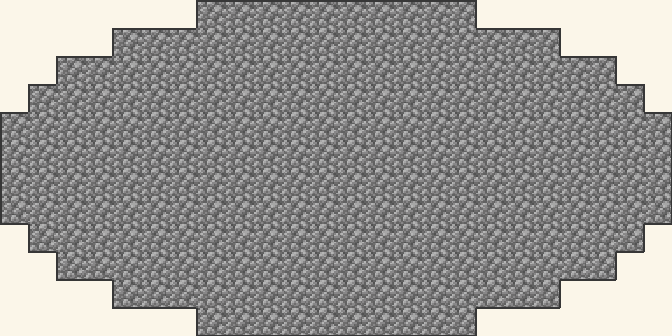
\includegraphics[width=0.45\textwidth]{fig07_2d_ellipse_24x12.png}
\caption{Ellipse $W = 24, H = 12$ dans Block Round. Notez que les cellules le long du grand axe sont plus espacees que le long du petit axe.}
\label{fig:elipse}
\end{figure}

\begin{enumerate}[leftmargin=1.5em,itemsep=0.15em,topsep=0.3em]
  \item Changer la forme pour \acc{Ellipse}. Deux \emph{sliders} apparaissent : \emph{Width} et \emph{Height}.
  \item Definir $W = 24$, $H = 12$. Observer la forme allongee --- voir Figure~\ref{fig:elipse}.
  \item Discuter : \emph{\enquote{L'equation qui regit cette forme est $(x/12)^2 + (y/6)^2 = 1$. Pourquoi divise-t-on $x$ par $12$ et $y$ par $6$ ?}}
\end{enumerate}

\subsection{Mode 3D, sphere et ellipsoide}

\begin{enumerate}[leftmargin=1.5em,itemsep=0.15em,topsep=0.3em]
  \item Changer le mode pour \acc{3D / Sphere}, taille $D = 12$.
  \item Faire glisser avec la \emph{souris} pour faire tourner. Apparait une sphere composee de voxels.
  \item Activer l'\emph{Info chip} : noter le volume (\enquote{904 blocks $= 14 \times 64 + 8$}).
  \item Passer a \acc{Ellipsoid}, $W = 20$, $H = 10$, $D = 12$.
  \item Demontrer le \emph{slider} \emph{Cut} sur l'axe \texttt{Y}, 50~\% (voir Figure~\ref{fig:cortes}~(a)). Observer la moitie superieure disparaitre.
  \item Alterner avec l'axe diagonal $\swarrow$/$\nearrow$ ($45^\circ$, Figure~\ref{fig:cortes}~(c)). Discuter la coupe oblique.
\end{enumerate}

\subsection{Exportation vers Minecraft}
\begin{enumerate}[leftmargin=1.5em,itemsep=0.15em,topsep=0.3em]
  \item Montrer le bouton de \emph{download} dans le coin du canvas : PNG.
  \item Montrer le bouton d'\emph{export schematic} : enregistre un fichier \texttt{.schem} au format Sponge v2.
  \item Demontrer (si possible) l'importation dans Minecraft Java via le mod Litematica. Voir Annexe~\ref{ap:litematica}.
\end{enumerate}

% =============================================================================
\newpage
\section{Liste d'exercices}\label{ap:exerc}

\textbf{Consignes :} repondre individuellement. On peut consulter Block Round pour confirmer les reponses, \emph{mais la justification mathematique est obligatoire}. Remettre manuscrit ou dactylographie.

\subsection*{Exercice 1 --- Equation du cercle}
\textbf{Enonce :} Considerer un cercle centre a l'origine $(0, 0)$ de rayon $r = 7$. Verifier si chacun des points suivants se trouve \emph{a l'interieur}, \emph{a l'exterieur} ou \emph{sur} le cercle. Justifier avec l'equation.
\begin{enumerate}[label=\alph*),leftmargin=1.5em,itemsep=0.1em,topsep=0.2em,nosep]
  \item $(3, 4)$ \hfill \emph{corrige :} a l'interieur ($9 + 16 = 25 < 49$).
  \item $(5, 5)$ \hfill \emph{corrige :} \acc{a l'exterieur} ($25 + 25 = 50 > 49$, car $\sqrt{50} \approx 7{,}07$).
  \item $(0, 7)$ \hfill \emph{corrige :} sur le cercle.
  \item $(-7, 0)$ \hfill \emph{corrige :} sur le cercle.
\end{enumerate}

\textit{Attention pedagogique :} l'item (b) est un piege deliberement pose.

\subsection*{Exercice 2 --- Arithmetique des piles et coffres}
\textbf{Enonce :} Considerer une sphere $D = 8$ en algorithme euclidien, de volume continu $V = \tfrac{4}{3}\pi \cdot 4^3 \approx 268{,}1$ et de volume discret $V_{\mathrm{disc}} = 268$.
\begin{enumerate}[label=\alph*),leftmargin=1.5em,itemsep=0.1em,topsep=0.2em,nosep]
  \item Combien de piles de cobblestone faut-il pour la construire ? Repondre sous la forme $q$ piles $+$ $r$ blocs supplementaires.
  \item Combien de coffres simples (27~emplacements) faut-il pour stocker toutes ces piles ?
  \item En mode survie, en supposant la collecte d'1~bloc toutes les 0{,}5~seconde avec une pioche en fer, quel est le temps total de collecte ?
\end{enumerate}

\emph{Corrige :} (a) $268 = 4 \times 64 + 12$, soit \acc{4 piles completes $+$ 12 blocs supplementaires} (5 emplacements dans l'inventaire). (b) 1 coffre simple suffit (27 emplacements, seuls 5 sont occupes). (c) $268 \times 0{,}5 = 134$ secondes $\approx$ 2~min 14~s.

\subsection*{Exercice 3 --- Comparaison d'algorithmes pour $D=20$}
\textbf{Enonce :} Sur Block Round, generer un cercle de diametre $D = 20$ dans les trois algorithmes.
\begin{enumerate}[label=\alph*),leftmargin=1.5em,itemsep=0.1em,topsep=0.2em,nosep]
  \item Noter l'aire (nombre de blocs) de chaque algorithme.
  \item Quel algorithme minimise le materiau ? Lequel le maximise ?
  \item Difference en \emph{piles} entre le plus grand et le plus petit ? Vaut-il la peine de choisir le plus petit pour economiser ?
\end{enumerate}

\emph{Corrige attendu :} Euclidien $\approx 316$~blocs (4 piles + 60 sup.), Bresenham $\approx 316$, Seuil $\approx 332$~blocs (5 piles + 12 sup.). Difference : $\approx 1$~pile. Sur un grand projet (spheres $D \geq 32$), l'economie se cumule.

\subsection*{Exercice 4 --- Volume d'une coupole et stockage}
\textbf{Enonce :} Considerer une sphere $D = 16$, algorithme Euclidien, coupee en Y a 50~\% (coupole classique).
\begin{enumerate}[label=\alph*),leftmargin=1.5em,itemsep=0.1em,topsep=0.2em,nosep]
  \item Volume continu de la sphere complete.
  \item Volume de la coupole (moitie superieure).
  \item Combien de coffres doubles faut-il pour stocker tous les blocs de la coupole ?
  \item Reste-t-il de quoi construire une partie du sol (une couche plane $16 \times 16$ blocs sous la coupole) ?
\end{enumerate}

\emph{Corrige :}
(a) $V = \tfrac{4}{3}\pi \cdot 8^3 \approx 2\,144{,}66$, $V_{\mathrm{disc}} \approx 2\,145$. (b) $V_{\mathrm{coupole}} \approx 1\,095$. (c) $\lceil 1\,095 / 3\,456 \rceil = 1$~coffre double. (d) Il reste : $3\,456 - 1\,095 = 2\,361$~blocs. Sol $16 \times 16 = 256$~blocs. Il reste $2\,105$~blocs --- on peut construire le sol et encore une couche de paillasse.

\subsection*{Exercice 5 --- Ellipsoide \enquote{table ronde geante}}
\textbf{Enonce :} Considerer un ellipsoide avec $W = 24$, $H = 8$, $D = 24$ (forme aplatie type \enquote{table}).
\begin{enumerate}[label=\alph*),leftmargin=1.5em,itemsep=0.1em,topsep=0.2em,nosep]
  \item Volume continu.
  \item Volume discret estime dans Block Round.
  \item Reste-t-il ou manque-t-il du materiau si l'on a achete 3~coffres doubles d'Oak Planks ?
\end{enumerate}

\emph{Corrige :}
(a) $V = \tfrac{4}{3}\pi \cdot 12 \cdot 4 \cdot 12 \approx 2\,413$.
(b) $V_{\mathrm{disc}} \approx 2\,400$ (varie de $\pm 10$ selon l'algorithme).
(c) Capacite achetee : $3 \times 3\,456 = 10\,368$~blocs. Il reste beaucoup --- $\approx 8\,000$~blocs supplementaires. \emph{Achat exagere.} L'ideal serait 1~coffre double (reste $\approx 1\,000$~blocs).

\subsection*{Exercice 6 --- WorldEdit vs Block Round}
\textbf{Enonce :} La commande WorldEdit \cmd{//sphere stone 15} utilise un algorithme similaire au Bresenham 3D. Comparer avec la sortie de Block Round en mode Bresenham pour $D = 30$ :
\begin{enumerate}[label=\alph*),leftmargin=1.5em,itemsep=0.1em,topsep=0.2em,nosep]
  \item Doivent-ils etre identiques ?
  \item S'ils ne le sont pas, pourquoi ? Lister au moins deux raisons.
\end{enumerate}

\emph{Corrige :}
(a) \emph{Approximativement oui} --- les deux sont Bresenham 3D, mais (b) ils peuvent differer en raison de : (i) implementations differentes (Block Round est en JavaScript ; WorldEdit est en Java) ; (ii) traitement de la parite du diametre (pair vs impair) ; (iii) constante empirique de \emph{seuil} (si l'un des deux utilise Seuil en interne). Difference typique : 0--6~blocs pour $D = 30$.

\subsection*{Exercice 7 --- Construction par symetrie octaedrique}
\textbf{Enonce :} Projeter la construction d'une sphere $D = 16$ centree en $(0, 72, 0)$ dans Minecraft, en utilisant la symetrie. Construire 1~octant (region $+x, +y, +z$, $\approx 268$~blocs) et refleter 7~fois via \cmd{/clone}.
\begin{enumerate}[label=\alph*),leftmargin=1.5em,itemsep=0.1em,topsep=0.2em,nosep]
  \item Ecrire les 7~commandes \cmd{/clone} (utiliser \cmd{mode:masked} pour ne pas effacer le terrain).
  \item Calculer le temps total estime : construction manuelle de l'octant + commandes.
\end{enumerate}

\emph{Corrige :}

\begin{minecraft}[Sequence de commandes]
\cmd{/clone 0 72 0 7 79 7 -8 72 0 mode:masked} \quad (refl.\ $-x$)\\
\cmd{/clone 0 72 0 7 79 7 0 64 0 mode:masked} \quad\quad (refl.\ $-y$)\\
\cmd{/clone 0 72 0 7 79 7 0 72 -8 mode:masked} \quad (refl.\ $-z$)\\
\cmd{/clone -8 72 0 -1 79 7 mode:masked} \quad\quad\;\; (octant $-x,-y$)\\
\cmd{/clone 0 64 -8 7 71 -1 mode:masked} \quad\quad\;\; (octant $-y,-z$)\\
\cmd{/clone -8 72 -8 -1 79 -1 mode:masked} \quad\;\; (octant $-x,-z$)\\
\cmd{/clone -8 64 -8 -1 71 -1 mode:masked} \quad\;\; (octant $-x,-y,-z$)
\end{minecraft}

Temps : $\sim$\,5~min (octant manuel en survie) + $\sim$\,3~s (7~clones).

\subsection*{Exercice 8 --- Projet final}
\textbf{Enonce :} Apres avoir produit la construction en groupe (Activite~\ref{at:53}), repondre :
\begin{enumerate}[label=(\arabic*),leftmargin=1.7em,itemsep=0.15em,topsep=0.2em,nosep]
  \item Lister les figures geometriques utilisees (cercle, ellipse, sphere, ellipsoide) et leurs parametres (diametre ou demi-axes).
  \item Pour la figure principale, quel algorithme a ete choisi ? Pourquoi ? Quel effet visuel produit-il que les deux autres ne produiraient pas ?
  \item Y a-t-il eu des coupes 3D ? Si oui, decrire mathematiquement \emph{l'une d'entre elles} comme inegalite.
  \item Combien de piles / coffres faudrait-il pour la construire reellement dans Minecraft en survie ?
  \item Votre production dialogue-t-elle avec une reference culturelle francaise (modernite, art geometrique, patrimoine vernaculaire, architecture de Le Corbusier, communaute francophone de Minecraft) ? Commenter.
\end{enumerate}

% =============================================================================
\newpage
\section{Adaptation aux lycees sans salle informatique}\label{ap:adapt-analog}

Cette adaptation permet d'appliquer la sequence \emph{integralement sur papier} lorsque l'acces a un ordinateur est rendu impossible --- realite frequente dans certains lycees ruraux, dans des contextes d'urgence sociale ou dans les REP/REP+ a fort taux de rotation des materiels. Le fil conceptuel reste intact ; ce qui change, c'est le support materiel.

\subsection{Substitutions par seance}

\begin{center}
\small
\begin{tabularx}{\textwidth}{@{}p{0.13\textwidth}p{0.32\textwidth}X@{}}
\toprule
\textbf{Seance} & \textbf{Activite d'origine} & \textbf{Adaptation analogique} \\
\midrule
1 & Demonstration de Block Round (1.3) & L'enseignant\textperiodcentered e dessine a la main trois versions du cercle $D = 10$ sur une grille pre-imprimee a la taille du tableau --- une par algorithme. Les Figures~\ref{fig:comp-d10} et~\ref{fig:comp-d20} peuvent etre imprimees comme reference. \\
\addlinespace[3pt]
2 & Comparaison quantitative sur logiciel (\ref{at:25}) & Distribuer des feuilles avec les trois cercles $D = 16$ pre-dessines et demander un comptage manuel. \\
\addlinespace[3pt]
3 & Generation de la sphere 3D (\ref{at:31},~\ref{at:32}) & Distribuer des feuilles avec des \emph{tranches} de la sphere ($z = 0, 1, 2, \ldots$) sur papier quadrille. L'eleve construit le modele mental par empilement. Chaque feuille simule une \emph{couche} de blocs Minecraft. \\
\addlinespace[3pt]
4 & Commandes Minecraft (\ref{at:42}) & Remplacer les commandes par des \emph{instructions de construction} ecrites en francais ; les eleves simulent l'execution sur papier quadrille. \\
\addlinespace[3pt]
5 & Construction reelle dans Minecraft (\ref{at:53}) & Construction en \emph{LEGO} (si disponible), sur papier quadrille colorie aux crayons vert-herbe et marron-terre, ou en \emph{cubes de papier} plies par les eleves en cours d'Arts plastiques. \\
\bottomrule
\end{tabularx}
\end{center}

\subsection{Feuilles auxiliaires}
Pour la version analogique complete, on recommande de preparer prealablement :
\begin{itemize}[leftmargin=1.3em,itemsep=0.1em,topsep=0.2em,nosep]
  \item 1 feuille A3 avec une grille $30 \times 30$ tracee a la regle.
  \item 1 jeu par eleve de 5 feuilles A4 quadrillees (5~mm).
  \item 1 feuille avec les trois cercles comparatifs pre-imprimes : les Figures~\ref{fig:comp-d10} et~\ref{fig:comp-d20} de ce document, en A4, servent de reference.
  \item Pour la Seance~5 analogique : 8~cubes de papier pre-plies par groupe (representant des blocs de cobblestone, oak, quartz, diamond).
\end{itemize}

\subsection{Valorisation des savoirs locaux}
Dans les lycees ruraux ou dans les territoires a forte tradition artisanale (tapisserie de Bayeux en Normandie, dentelle du Puy-en-Velay en Haute-Loire, faience de Quimper ou de Nevers, marqueterie d'Annecy, vitrail medieval de Chartres), la Seance~\ref{aula3} peut etre \emph{enrichie par une visite d'artisan\textperiodcentered e ou de porteur\textperiodcentered euse de savoir traditionnel} : dentellieres, tapissieres, ceramistes, maitres-verriers, montrant comment ils\textperiodcentered elles rasterisent des cercles dans leurs langages propres. Cette approche realise le principe ethnomathematique tout en mobilisant le patrimoine culturel et industriel francais. En outre-mer, articulation possible avec les artisans des cases creoles (Reunion, Martinique, Guadeloupe), des fare (Polynesie), des cases kanak (Nouvelle-Caledonie).

% =============================================================================
\newpage
\section{Glossaire technique pour l'enseignant\textperiodcentered e}\label{ap:glos}

\begin{itemize}[leftmargin=1.4em,itemsep=0.3em,topsep=0.3em]
  \item \acc{Algorithme} --- sequence finie et bien definie d'instructions pour resoudre un probleme. Les trois algorithmes de Block Round (cf.\ Figure~\ref{fig:comp-d10}) sont des procedures distinctes pour le meme probleme.
  \item \acc{Coffre (simple)} --- conteneur Minecraft a 27~emplacements. Capacite : $27 \times 64 = 1\,728$~articles.
  \item \acc{Coffre double} --- deux coffres adjacents qui se combinent en un conteneur de 54~emplacements. Capacite : $54 \times 64 = 3\,456$~articles.
  \item \acc{Bloc} --- unite de construction de Minecraft. Cube $1\times1\times1$ a six faces texturees. En langage mathematique, c'est un \emph{voxel}.
  \item \acc{Bresenham (algorithme de)} --- algorithme publie en 1965 par Jack Bresenham (IBM), originellement pour la droite, etendu par d'autres auteurs (Pitteway, Kappel) pour l'ellipse. Sa marque est de n'utiliser \emph{que des entiers}. Voir Activite~\ref{at:23}.
  \item \acc{BO} --- \emph{Bulletin Officiel} de l'Education nationale, qui publie le programme de specialite Mathematiques (22~janvier 2019, modifie 2022).
  \item \acc{Canvas} --- element HTML qui propose un espace de dessin 2D ou 3D dans le navigateur.
  \item \acc{\code{/clone}} --- commande vanilla de Minecraft qui copie une region rectangulaire vers une autre position. Syntaxe : \cmd{/clone x1 y1 z1 x2 y2 z2 dx dy dz}. Essentielle pour la construction par symetrie.
  \item \acc{CRCN} --- Cadre de Reference des Competences Numeriques. Definit les competences PIX requises pour la certification.
  \item \acc{Equation implicite} --- equation de la forme $F(x, y) = 0$. Celle de l'ellipse : $(x/r_x)^2 + (y/r_y)^2 - 1 = 0$.
  \item \acc{Ethnomathematique} --- domaine fonde par le bresilien Ubiratan D'Ambrosio (traduit au CNRS).
  \item \acc{\code{/fill}} --- commande vanilla de Minecraft qui remplit une boite rectangulaire avec un type de bloc. Syntaxe : \cmd{/fill x1 y1 z1 x2 y2 z2 minecraft:stone}.
  \item \acc{Grand Oral} --- epreuve du Baccalaureat general (depuis 2021) ou un\textperiodcentered e eleve presente, pendant 20~minutes, un sujet articulant deux de ses specialites.
  \item \acc{IHES} --- Institut des Hautes Etudes Scientifiques (Bures-sur-Yvette, \url{https://www.ihes.fr/}). Centre de recherche mondial de premier plan ; modele inspire de Princeton IAS.
  \item \acc{IREM} --- Institut de Recherche sur l'Enseignement des Mathematiques, present dans chaque academie.
  \item \acc{Litematica} --- mod populaire de Minecraft Java Edition qui importe les schematics et affiche un \emph{fantome} translucide de la construction a realiser bloc par bloc. Gratuit.
  \item \acc{Minecraft Education} --- version educative de Minecraft, gratuite pour les enseignants via Microsoft~365 Education.
  \item \acc{NSI} --- specialite \emph{Numerique et Sciences Informatiques}, enseignement de specialite du lycee general (creee en 2019).
  \item \acc{Pack / Pile} --- empilement d'au plus 64~blocs identiques dans un emplacement de l'inventaire de Minecraft.
  \item \acc{PIX} --- service public en ligne d'evaluation et de certification des competences numeriques (CRCN). Niveau attendu en fin de Terminale : niveau 5 a 6 sur 8.
  \item \acc{Pixel} --- abreviation de \emph{picture element}. En 2D.
  \item \acc{PWA} --- \emph{Progressive Web App}. Application \emph{web} installable et utilisable \emph{hors ligne}.
  \item \acc{Rasterisation} --- processus de conversion d'une description geometrique continue en une matrice de pixels (2D) ou de voxels (3D).
  \item \acc{RGPD} --- Reglement General sur la Protection des Donnees (UE 2016/679), encadre en France par la Loi Informatique et Libertes (1978, modifiee 2018), sous controle de la CNIL.
  \item \acc{Schematica} --- mod alternatif a Litematica, avec une fonction similaire.
  \item \acc{Schematic (\texttt{.schem})} --- format de fichier qui serialise une region de Minecraft (Sponge Schematic v2, gzip + NBT).
  \item \acc{Demi-axe} --- dans une ellipse, distance du centre a une extremite dans la direction de l'axe.
  \item \acc{\code{//sphere}} --- commande WorldEdit qui construit une sphere. Syntaxe : \cmd{//sphere bloc rayon}.
  \item \acc{Emplacement} --- cellule individuelle de l'inventaire de Minecraft. Inventaire complet du joueur : 36~emplacements ($9 \times 4$).
  \item \acc{Voxel} --- abreviation de \emph{volume element}. Generalisation du pixel a la 3D. Dans Minecraft, chaque \emph{bloc} est un voxel.
  \item \acc{WebGL} --- bibliotheque de programmation graphique 3D dans le navigateur.
  \item \acc{WorldEdit} --- mod tres populaire de Minecraft Java qui ajoute des commandes avancees de construction a grande echelle, dont \cmd{//sphere}, \cmd{//hsphere}, \cmd{//ellipsoid}, \cmd{//cyl}, \cmd{//schem load}.
\end{itemize}

% =============================================================================
\newpage
\section{Tutoriel : de Block Round a Minecraft via Litematica}\label{ap:litematica}

Cette annexe decrit le flux complet d'exportation de Block Round et d'importation dans Minecraft Java Edition en utilisant le mod \emph{Litematica}. Duree totale attendue : 15~minutes (premiere fois).

\subsection{Prerequis}
\begin{itemize}[leftmargin=1.3em,itemsep=0.1em,topsep=0.2em,nosep]
  \item Minecraft Java Edition (achat sur la \emph{Mojang Store} ; la version educative \emph{Minecraft Education} fonctionne aussi, avec ajustements).
  \item \emph{Fabric Loader} pour la version de Minecraft utilisee (en general la plus recente : \url{https://fabricmc.net/use/}).
  \item Mods : \emph{Fabric API} et \emph{Litematica} (\url{https://www.curseforge.com/minecraft/mc-mods/litematica}).
  \item Block Round ouvert dans le navigateur, avec la figure souhaitee deja produite.
\end{itemize}

\subsection{Etape 1 : exporter depuis Block Round}
\begin{enumerate}[leftmargin=1.5em,itemsep=0.15em,topsep=0.3em]
  \item Sur Block Round, configurer la figure souhaitee (mode, forme, diametre, algorithme, bloc, coupe). Verifier le volume sur l'\emph{Info chip}.
  \item Cliquer sur le bouton \emph{Export Schematic} (coin superieur droit du canvas, deuxieme icone). Un fichier \texttt{.schem} sera telecharge.
\end{enumerate}

\subsection{Etape 2 : installer Litematica}
\begin{enumerate}[leftmargin=1.5em,itemsep=0.15em,topsep=0.3em]
  \item Installer Fabric Loader pour la version de Minecraft utilisee.
  \item Telecharger \emph{Fabric API} et \emph{Litematica} pour la meme version de Minecraft. Placer les deux dans le repertoire \texttt{.minecraft/mods/}.
  \item Demarrer Minecraft avec le profil \emph{fabric-loader-x.y.z-1.20.x}.
\end{enumerate}

\subsection{Etape 3 : importer le schematic}
\begin{enumerate}[leftmargin=1.5em,itemsep=0.15em,topsep=0.3em]
  \item Placer le fichier \texttt{.schem} dans \texttt{.minecraft/schematics/} (ou dans le dossier par defaut de Litematica, defini dans la Configuration du mod).
  \item Dans un monde (creatif ou survie), appuyer sur \texttt{M} pour ouvrir le menu de Litematica.
  \item Cliquer sur \emph{Load Schematic} $\rightarrow$ selectionner le fichier $\rightarrow$ \emph{Load}.
  \item Le schematic apparait dans une liste. Cliquer dessus puis sur \emph{Placement} : le \enquote{fantome} translucide de la figure apparait dans le monde.
  \item Utiliser les controles de deplacement (\texttt{M} $\rightarrow$ \emph{Placements}) pour glisser le fantome a la position souhaitee. Pour un terrain plat, il suffit de placer le coin inferieur $(x_1, y_1, z_1)$ au sol.
\end{enumerate}

\subsection{Etape 4 : construire}
\begin{enumerate}[leftmargin=1.5em,itemsep=0.15em,topsep=0.3em]
  \item En \emph{Creatif} : voler au-dessus du fantome et placer chaque bloc la ou Litematica l'indique ; le mod confirme en vert les blocs corrects et marque en rouge toute erreur. La construction d'une sphere $D = 12$ prend $\approx$\,5~minutes.
  \item En \emph{Survie} : identique, mais il faut collecter les blocs avant. Utiliser le calcul de piles / coffres de l'Activite~\ref{at:41} pour planifier la collecte.
  \item Alternative : si le serveur a WorldEdit, utiliser \cmd{//schem load nom-fichier} suivi de \cmd{//paste -a} pour une construction instantanee.
\end{enumerate}

\subsection{Etape 5 : verification}
Litematica met en rouge tout bloc errone (manquant, du mauvais type, ou en mauvaise position). Utiliser le raccourci \texttt{Z} pour alterner entre \emph{visible} et \emph{invisible} le fantome, en comparant avec la construction reelle.

\subsection{Resolution des problemes courants}
\begin{itemize}[leftmargin=1.3em,itemsep=0.15em,topsep=0.3em,nosep]
  \item \emph{Le schematic n'apparait pas dans la liste :} verifier que le fichier se trouve dans le bon dossier, et que la version de Litematica est compatible avec celle de Minecraft.
  \item \emph{Blocs errones / apparaissent gris :} certains blocs du schematic Block Round peuvent ne pas etre disponibles dans le monde (ancienne version de Minecraft) ; ouvrir le schematic avec un editeur de texte pour verifier les noms.
  \item \emph{Le fantome flotte :} ajuster la position avec l'option \emph{Rotation / Mirror} dans le menu Placement. Pour les spheres, c'est indifferent ; pour les ellipses, ajuster la rotation.
\end{itemize}

\vspace{2em}
\begin{center}
\color{muted}\small\sffamily
--- fin de la sequence pedagogique ---
\end{center}

\end{document}
